\documentclass[12pt]{article}

% Packages
\usepackage[utf8]{inputenc}
\usepackage{amsmath, amssymb}
\usepackage{graphicx}
\usepackage{hyperref}
\usepackage{geometry}
\geometry{a4paper, margin=1in}

% Title and Author
\title{Teaching Transformers Arithmetic}
\author{Richard Yang}
\date{\today}

\begin{document}

\maketitle

\section{Introduction}
Recently, large language models like GPT3/4 have shown impressive mathematical capabilities,
despite not having been trained explicitly on such tasks.
Understanding how these arithmetical abilities develop could shed light on how these models learn more general tasks.

In this report, we focus on the emergence of addition skills.
We train a small (10.6M parameters) transformer on various datasets of addition problems and analyze the model's performance,
aiming to replicate the results of \cite{lee2023teaching}.
We confirm its findings, and investigate the model's learning process in more detail.


\section{Literature Review}
Our work is based primarily on the work of \cite{lee2023teaching}.
Their abstract states:
\begin{quote}
    This study investigates how small transformers, trained
    from random initialization, can efficiently learn arithmetic operations such as
    addition, multiplication, and elementary functions like square root, using the next-
    token prediction objective. We first demonstrate that conventional training data
    is not the most effective for arithmetic learning, and simple formatting changes
    can significantly improve accuracy \dots Building on prior work, we then train
    on chain-of-thought style data that includes intermediate step results \dots
    this approach significantly and simultaneously
    improves accuracy, sample complexity, and convergence speed. We also study
    the interplay between arithmetic and text data during training and examine the
    effects of few-shot prompting, pretraining, and model scale. Additionally, we
    discuss length generalization challenges. Our work highlights the importance of
    high-quality, instructive data that considers the particular characteristics of the
    next-word prediction objective for rapidly eliciting arithmetic capabilities.
\end{quote}
Some related work includes:
\begin{itemize}
    \item Length Generalization in Arithmetic Transformers \cite{jelassi2023length}. This work uses relative position embeddings to improve length generalization, as well as introducing "train set priming" for multiplication tasks, allowing generalization to much longer inputs.
    \item Arithmetic transformers can length generalize in both operand length and count \cite{cho2024arithmetic}. This work achieves 2-3x length generalization on addition and multiplication by introducing task-specific scratchpads and multi-level position coupling.
    \item Teaching transformers modular arithmetic at scale \cite{saxena2024teaching}. Using angular embeddings and a custom loss function, this work enables transformeres to perform large scale modular arithmetic tasks, like summing 256 numbers moduluo 3329.
\end{itemize}

\section{Methodology}
\subsection{Model Architecture}
We start with a small transformer model, based off of NanoGPT \cite{nanogpt}.
For all runs, we use a 10.6M parameter model with 6 layers, 8 heads, and embedding dimension 384.
The model is trained on an next token prediction objective. 
\subsection{Datasets}
We have three datasets: one with 1-digit addition problems, one with 3 digit addition problems, and one with 3 digit addition problems where the sum is reversed.
Each dataset consists of a set of addition problems, each represented as a string.
Each line is a separate example.
Datasets were generated randomly using a simple script.
For single digit and three digit addition, each line is formatted plainly as $$A_1A_2...A_i+B_1B_2...B_i=C_1C_2...C_j,$$
where $A_i$, $B_i$, and $C_j$ are digits.
For reversed three digit addition, we have left padded the operands with zeros. The result is right padded with zeros, due to being reversed.
This ensures that each line has the same length.
\subsection{Data Loading}
We experiment with different data loading methods, to see their effect on the model's performance.
\begin{itemize}
    \item Random block sampling. Strings of the block size length are sampled at random from the dataset.
    \item Random line sampling. Lines of the dataset are sampled at random. We have only used this for the reversed three digit addition dataset.
\end{itemize}

\subsection{Model Evaluation}
During training, we periodically evaluate the model on a validation set.
For single digit addition, the validation set consists of all the 100 such problems.
For three digit addition and reversed three digit addition, the validation set consists of 1000 problems, randomly sampled from the test dataset.
The metrics we track are:
\begin{itemize}
    \item Simple accuracy. The number of correct predictions divided by the total number of predictions.
    \item Character accuracy. The number of correct characters found in the correct position divided by the total number of characters predicted.
    \item Individual position accuracy. The number of correct characters in a given position divided by the total number of characters in that position.
\end{itemize}
Instructions for running the evaluation script are in the code repository. Logging was done using wandb.
We are particularly interested in the character accuracy, and seeing if there is any structure in how the model learns to predict the digits.
\section{Results}
\subsection{Single Digit Addition}
\begin{figure}[h]
    \centering
    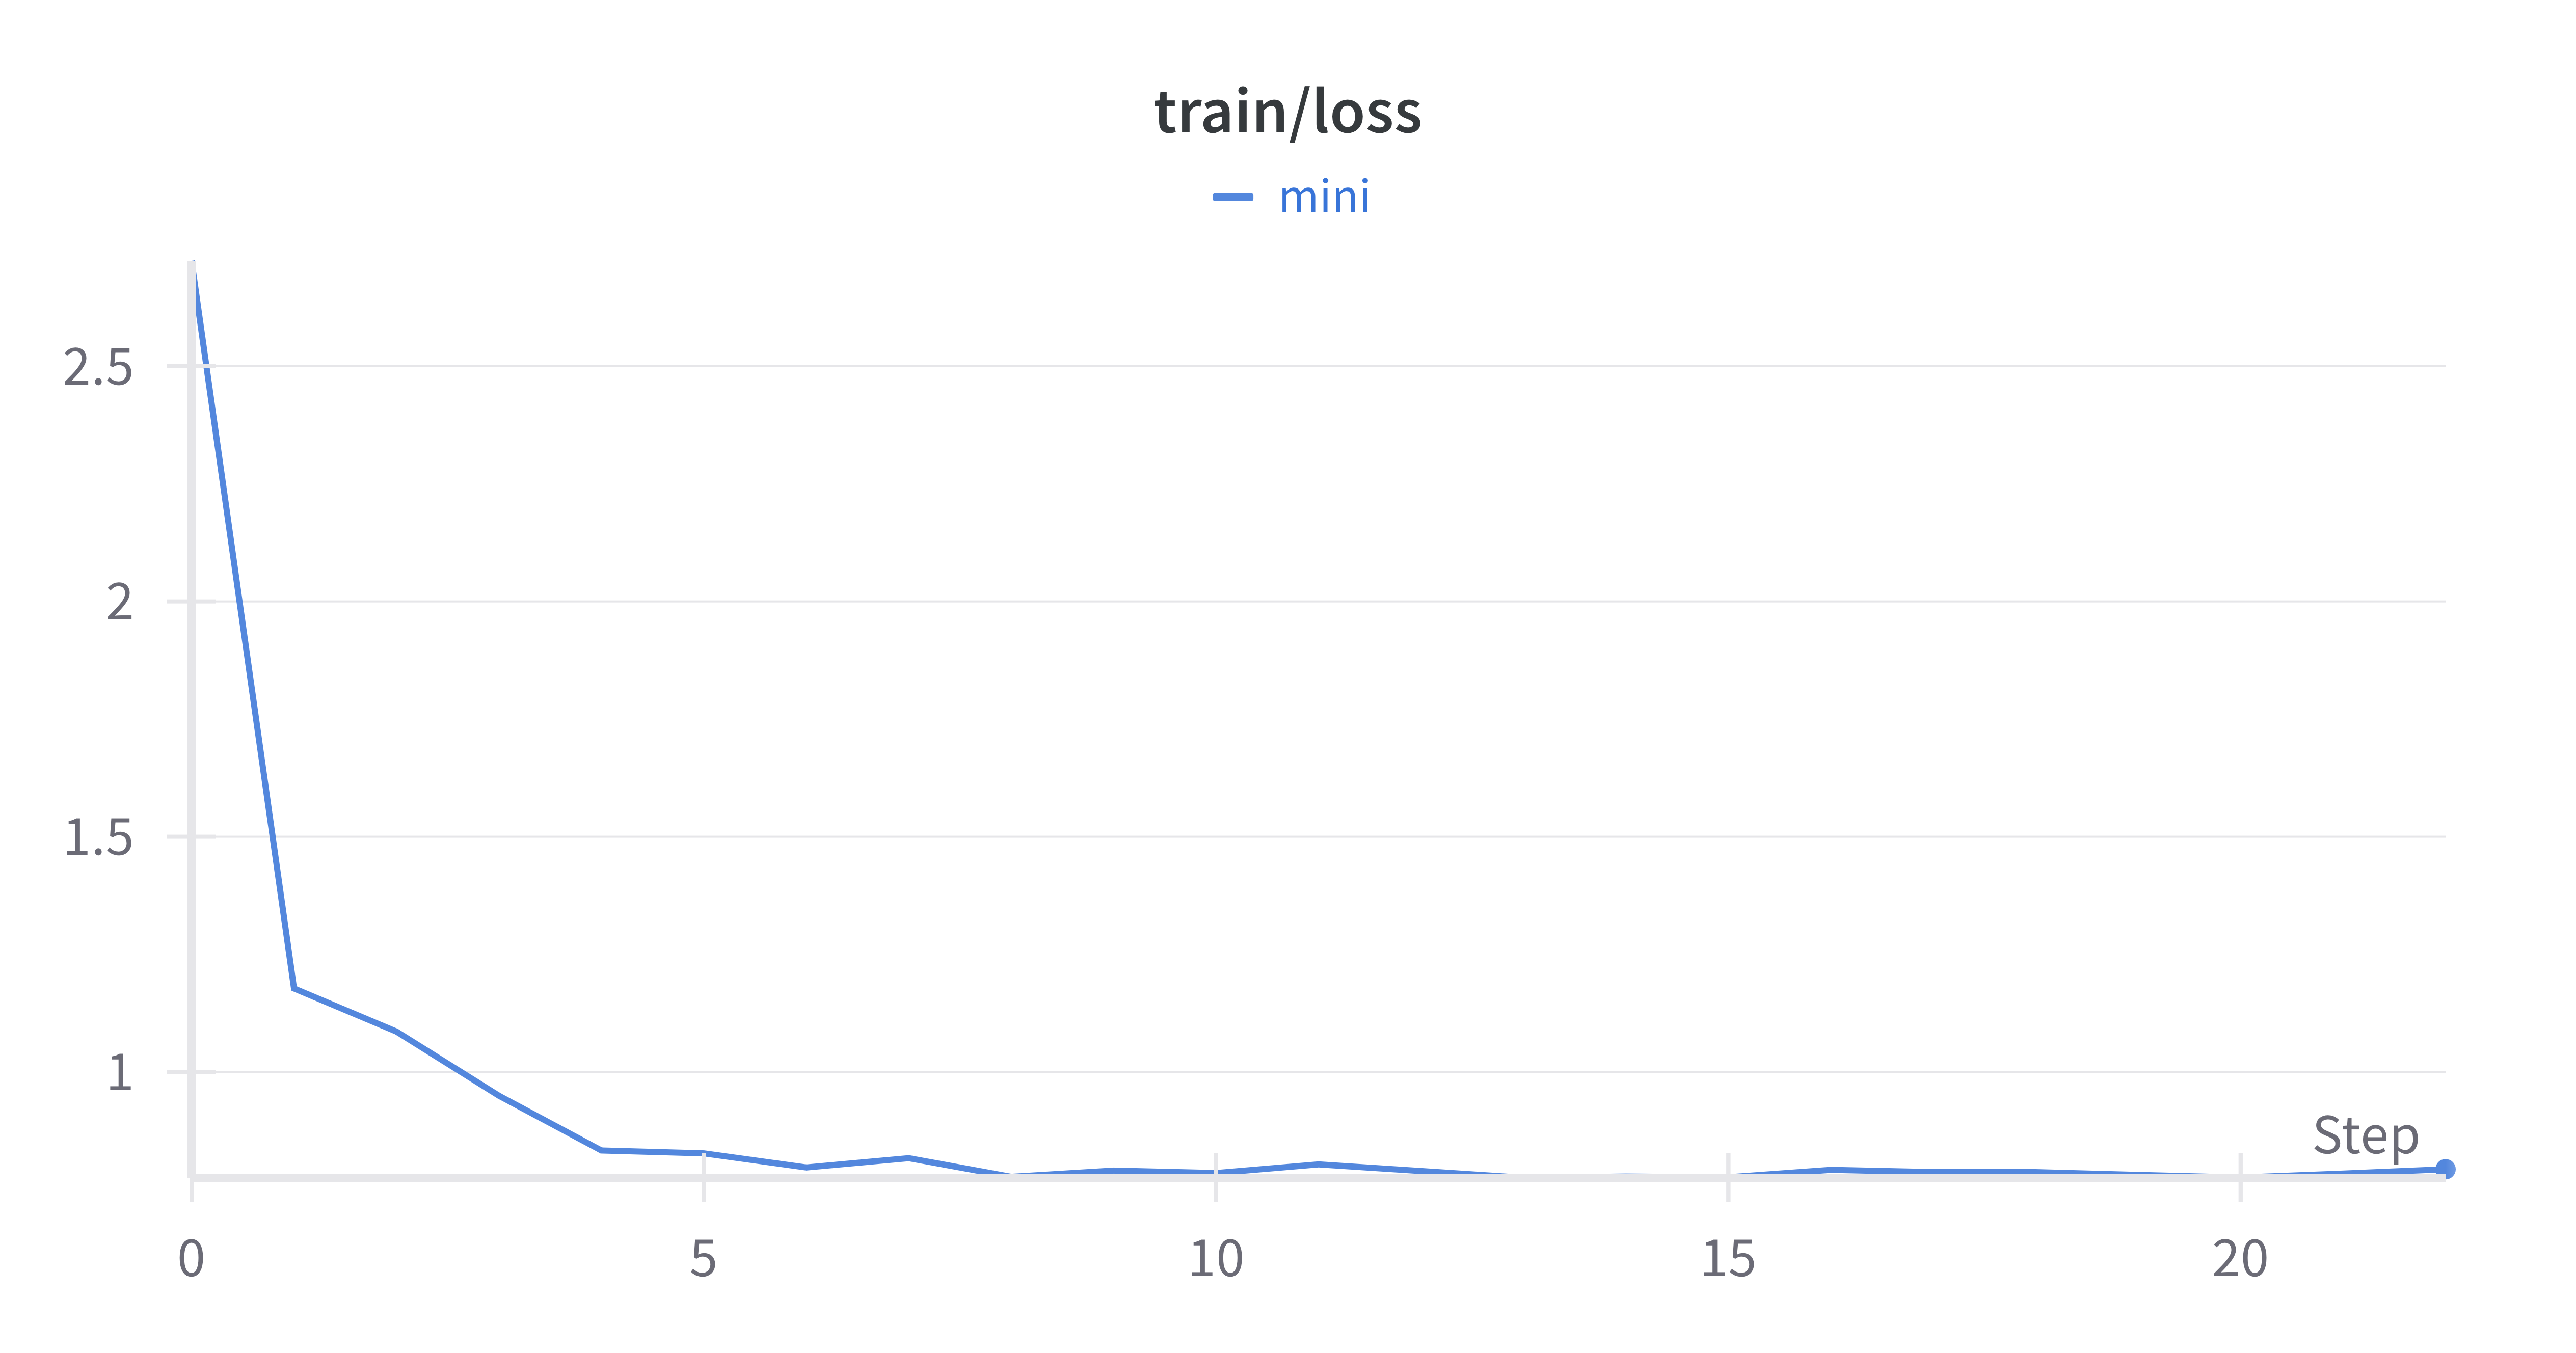
\includegraphics[width=0.5\textwidth]{figures/single-digit/single-digit-add-loss.png}
    \caption{Training loss.}
    \label{fig:single_digit_addition}
\end{figure}
\begin{figure}[h]
    \centering
    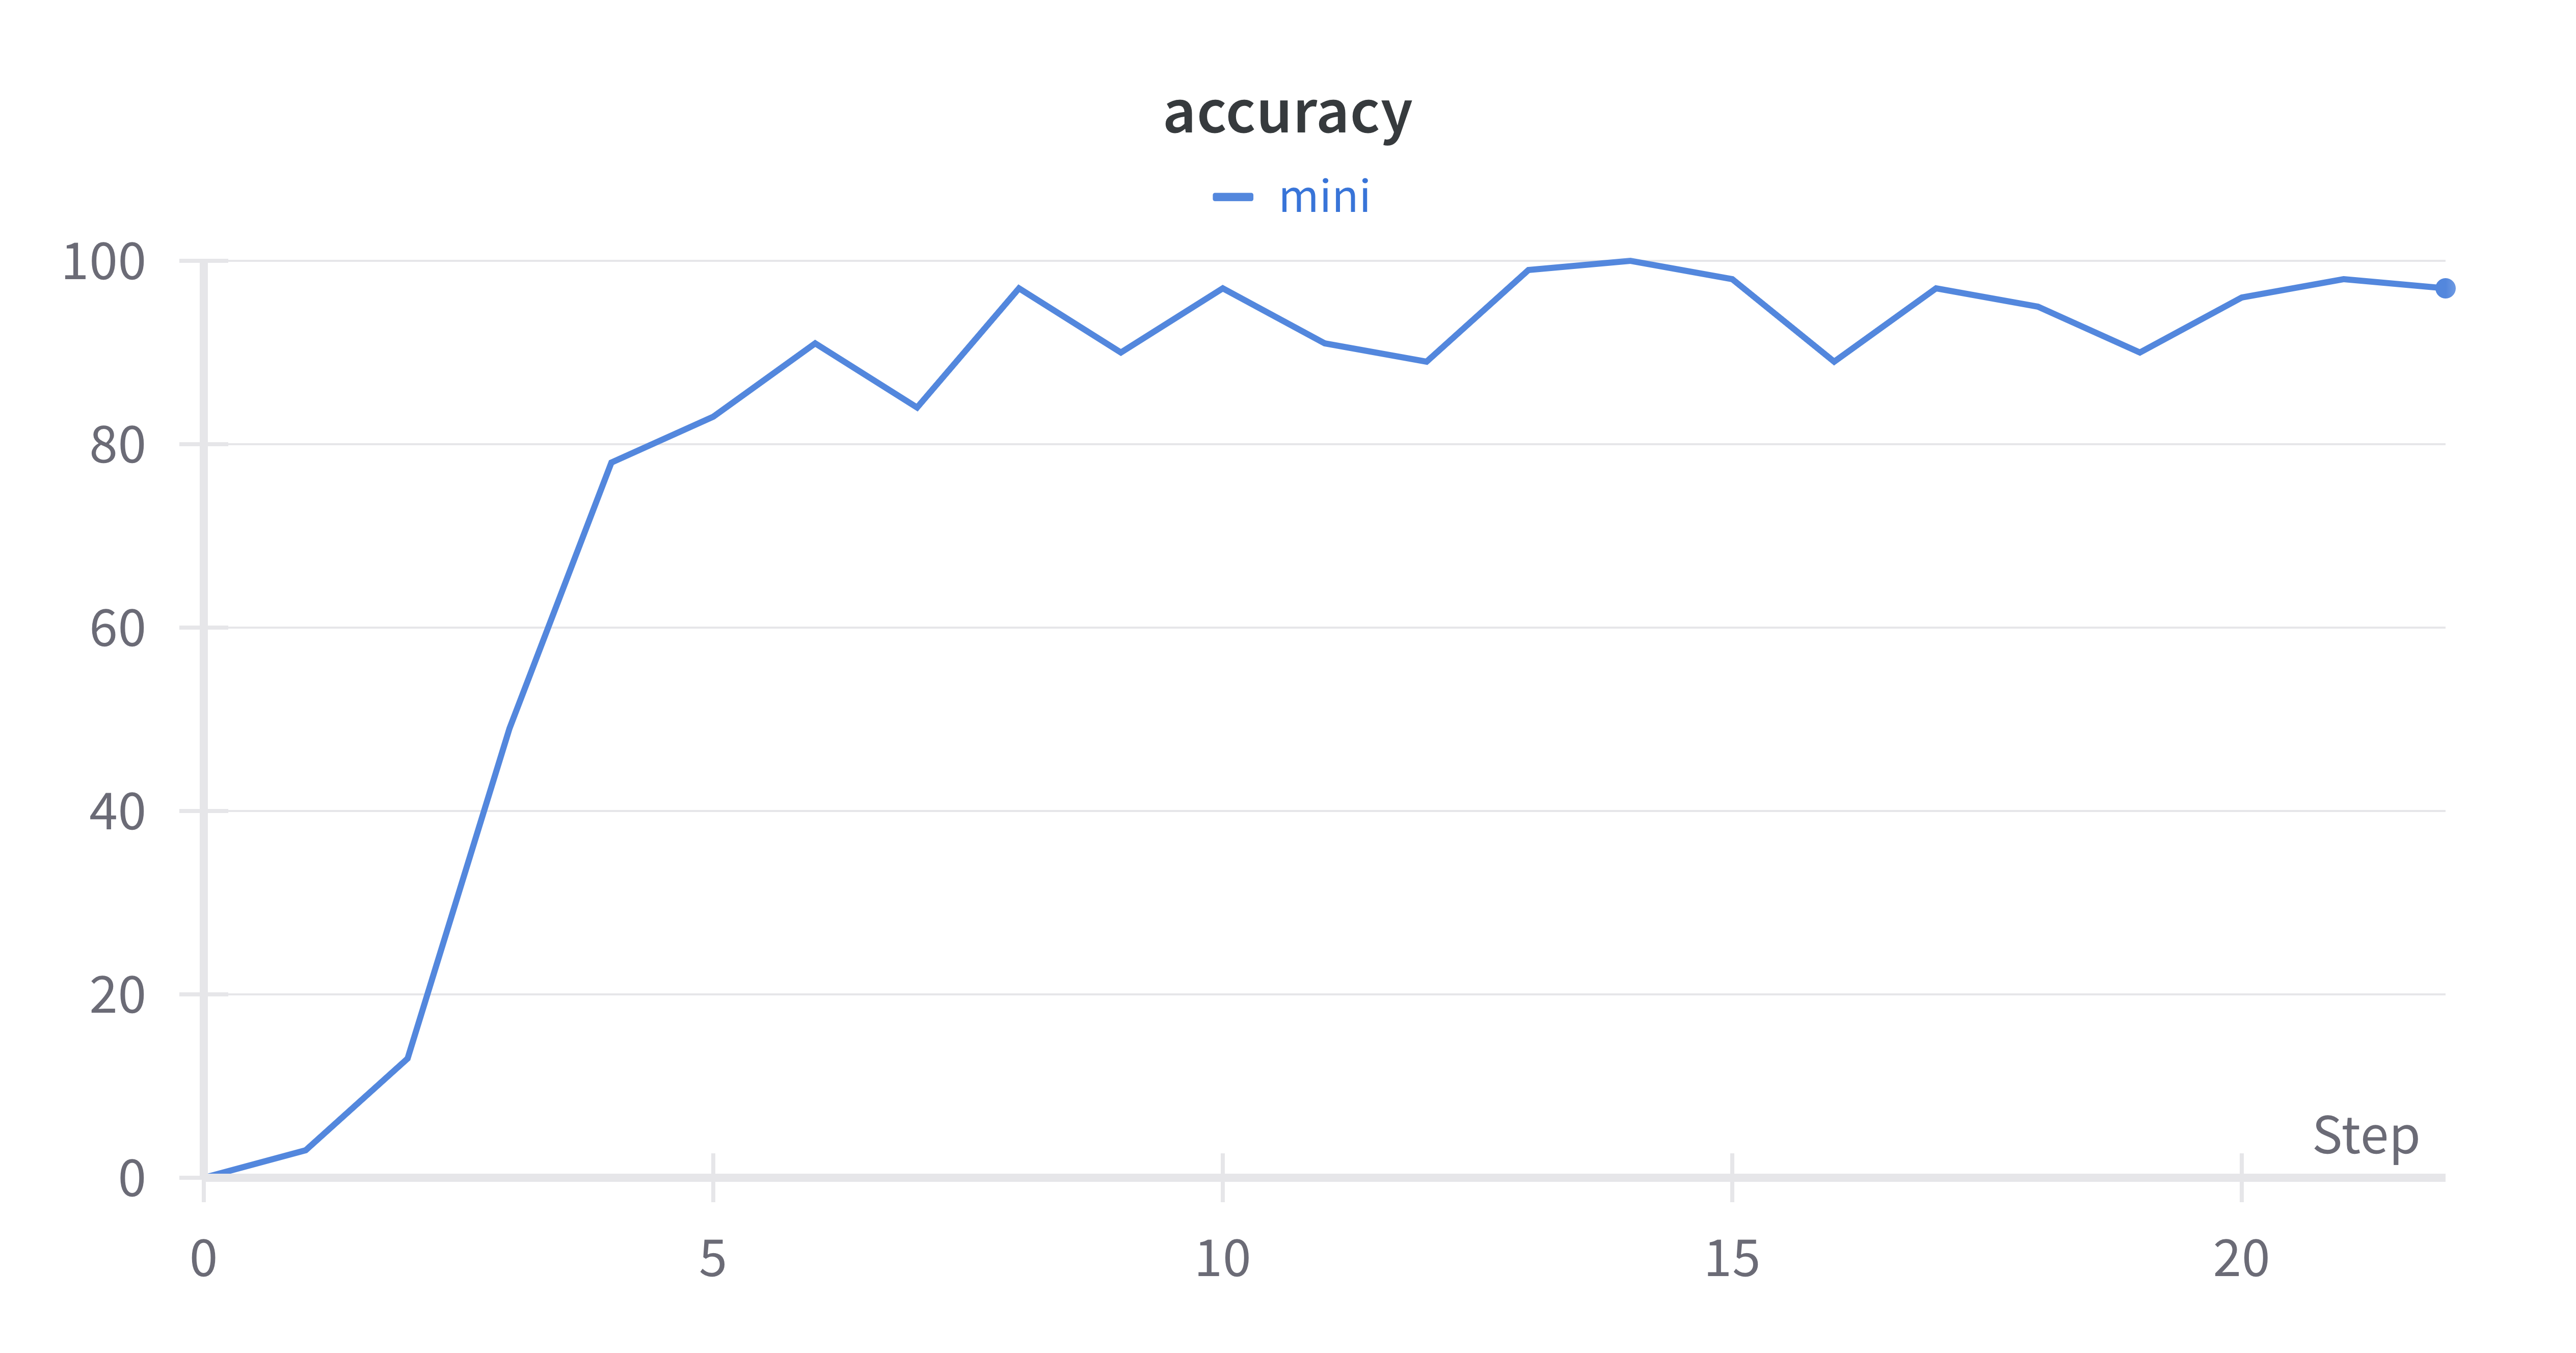
\includegraphics[width=0.5\textwidth]{figures/single-digit/single-digit-add-accuracy.png}
    \caption{Accuracy.}
    \label{fig:single_digit_addition_accuracy}
\end{figure}
\begin{figure}[h]
    \centering
    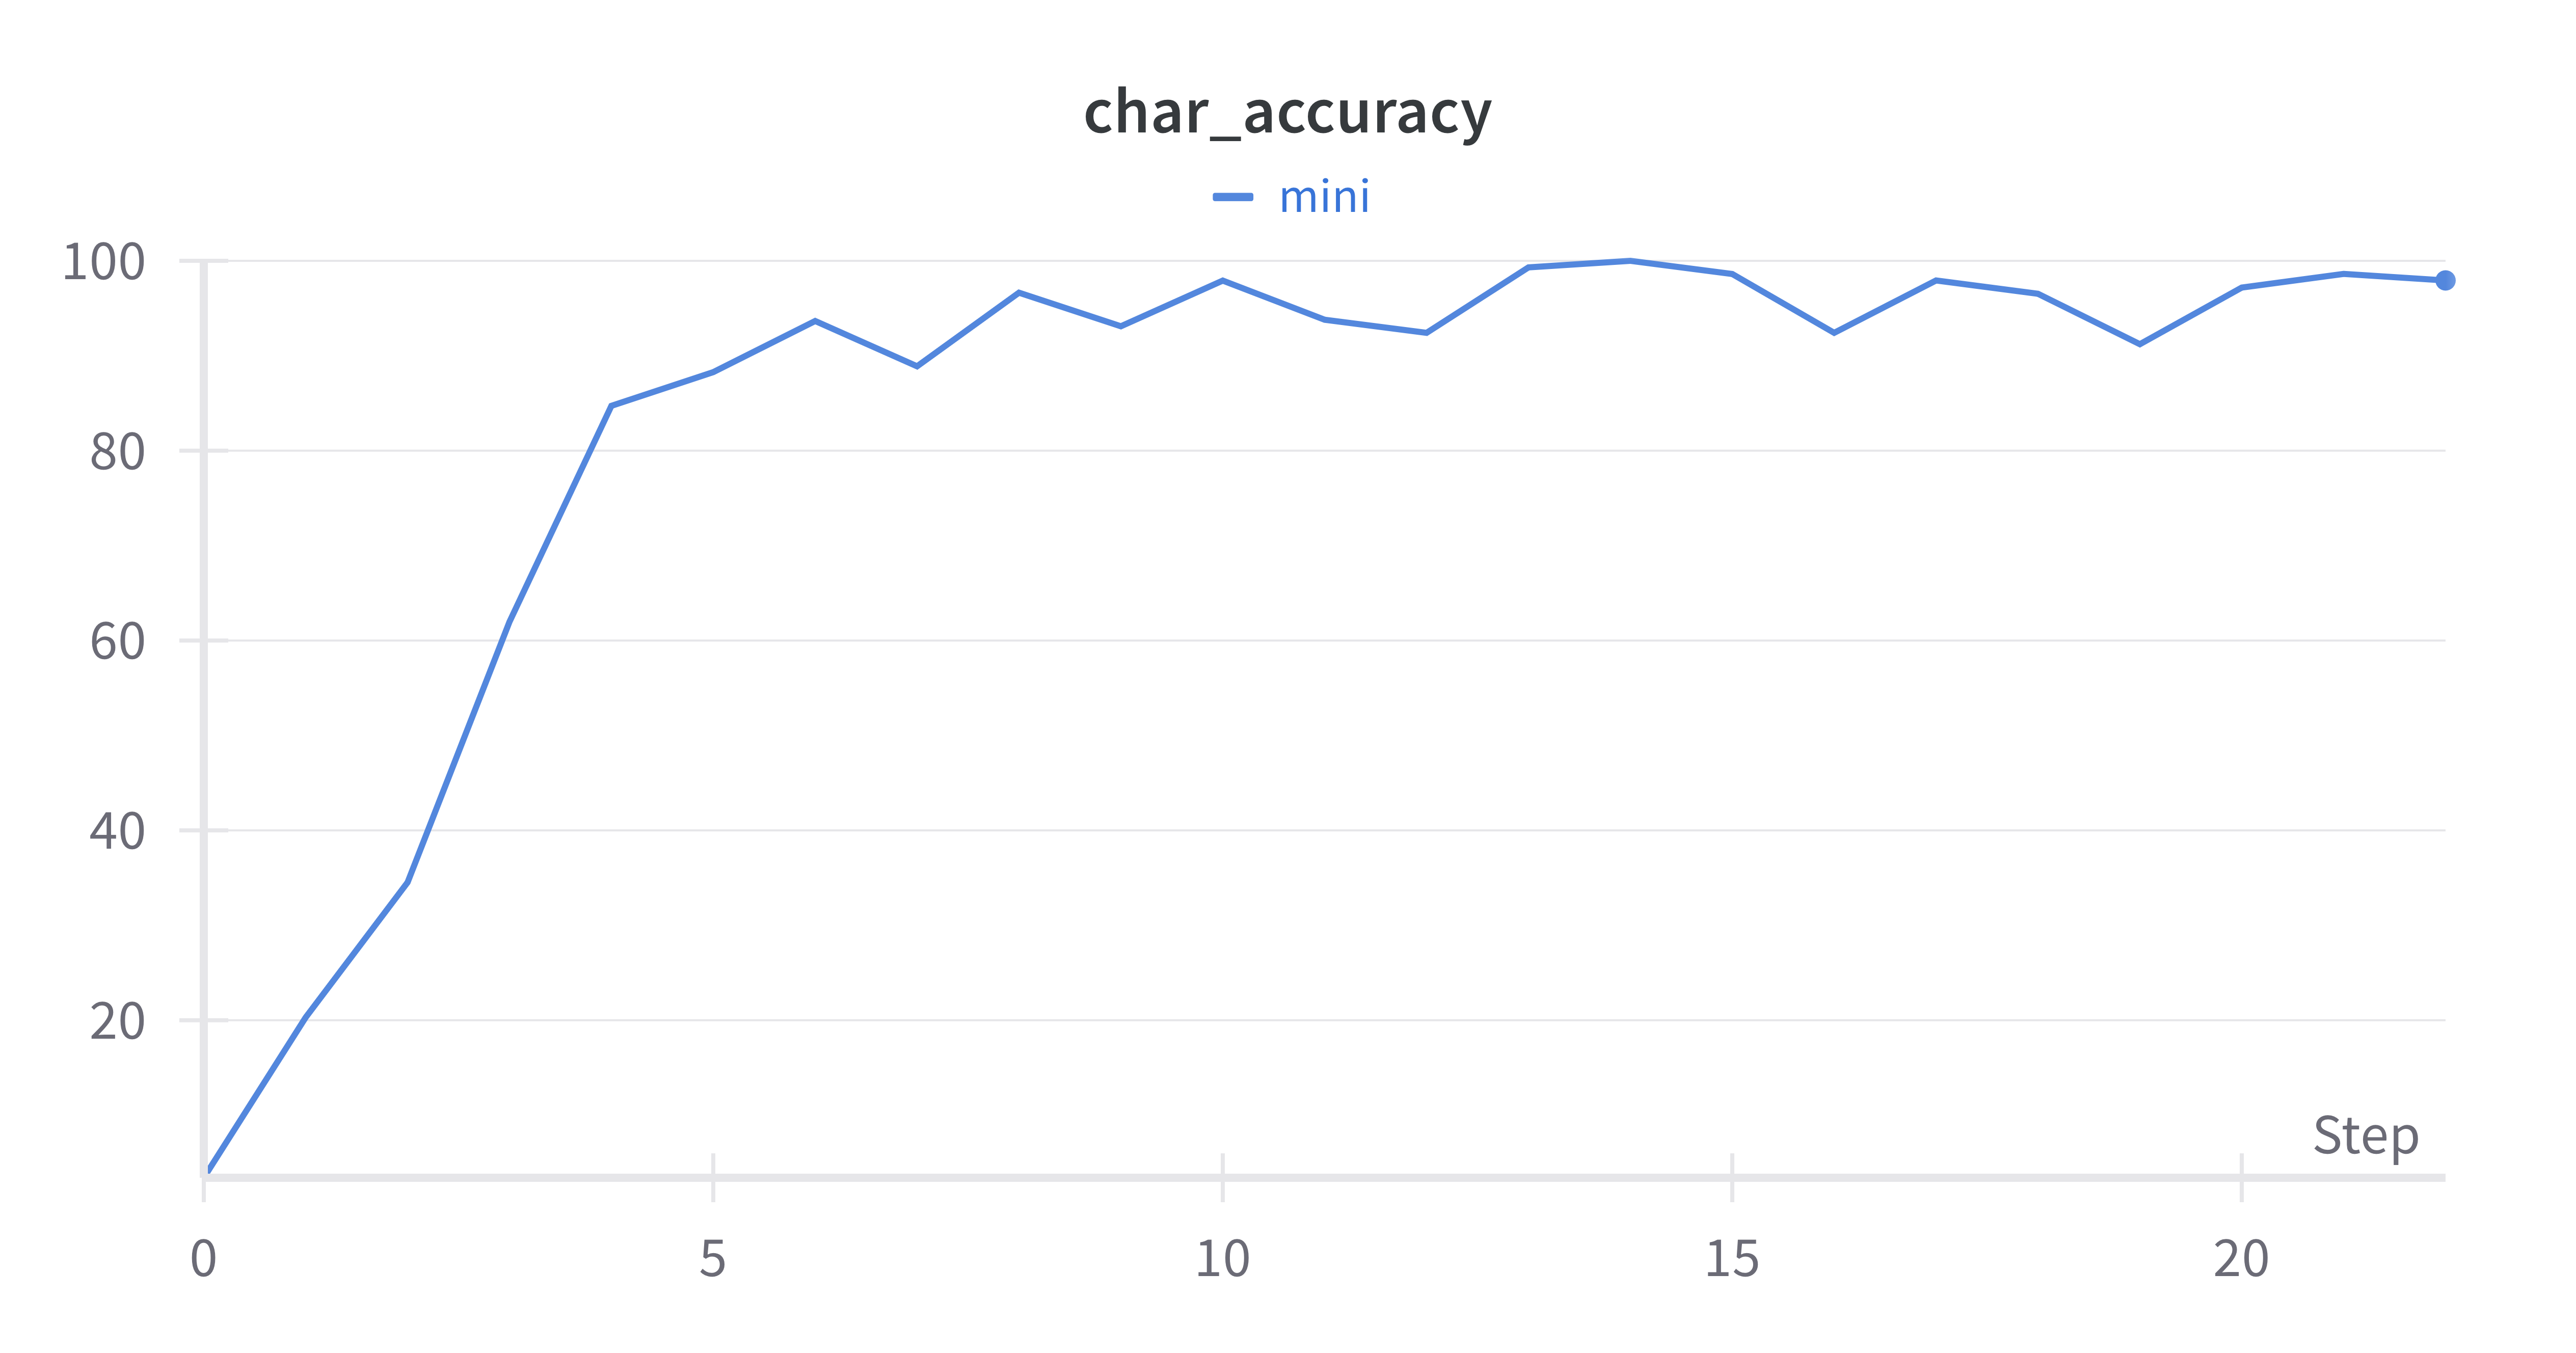
\includegraphics[width=0.5\textwidth]{figures/single-digit/single-digit-add-char-accuracy.png}
    \caption{Character accuracy.}
    \label{fig:single_digit_addition_char_accuracy}
\end{figure}
Figures for training loss, accuracy, and character accuracy are shown in Figures \ref{fig:single_digit_addition}, \ref{fig:single_digit_addition_accuracy}, and \ref{fig:single_digit_addition_char_accuracy} respectively.
Each step is 50 iterations.
It is apparent that accuracy increases exponentially at first, before plateauing around 90\%.
The character accuracy slightly leads the accuracy, as expected since there are only one or two digits in the answer.
\subsection{Three Digit Addition}
\begin{figure}[h]
    \centering
    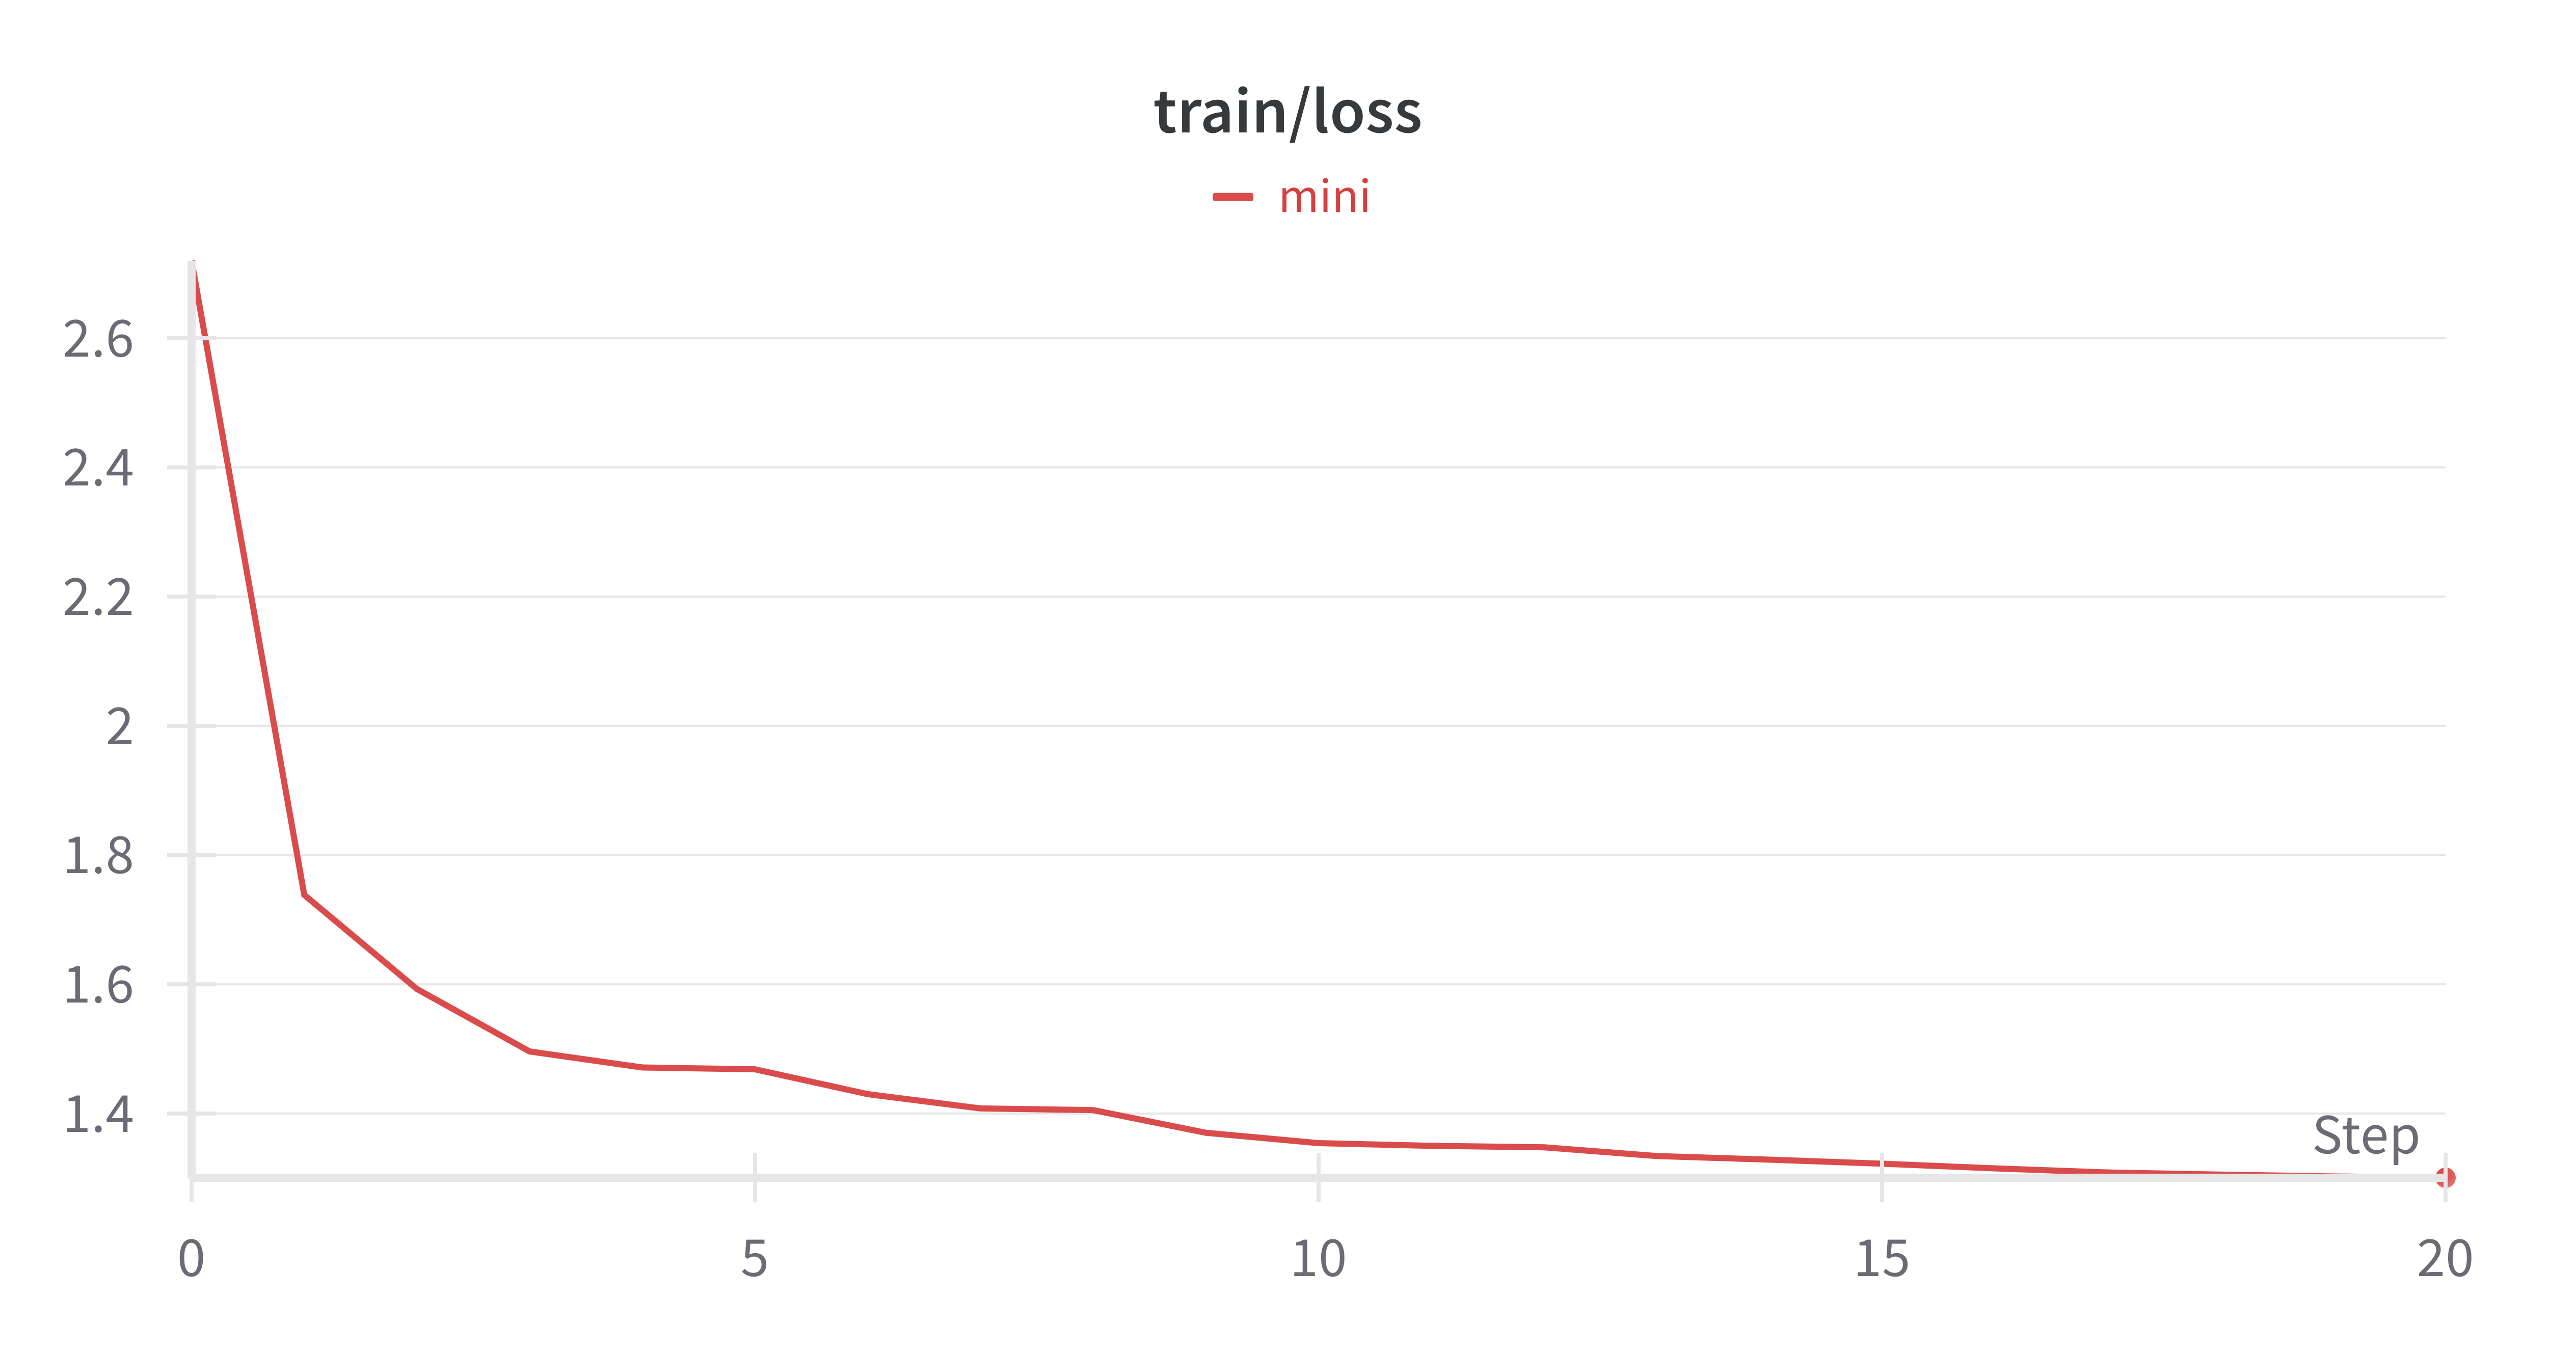
\includegraphics[width=0.5\textwidth]{figures/three-digit/three-digit-add-loss.png}
    \caption{Training loss.}
    \label{fig:three_digit_addition}
\end{figure}
\begin{figure}[h]
    \centering
    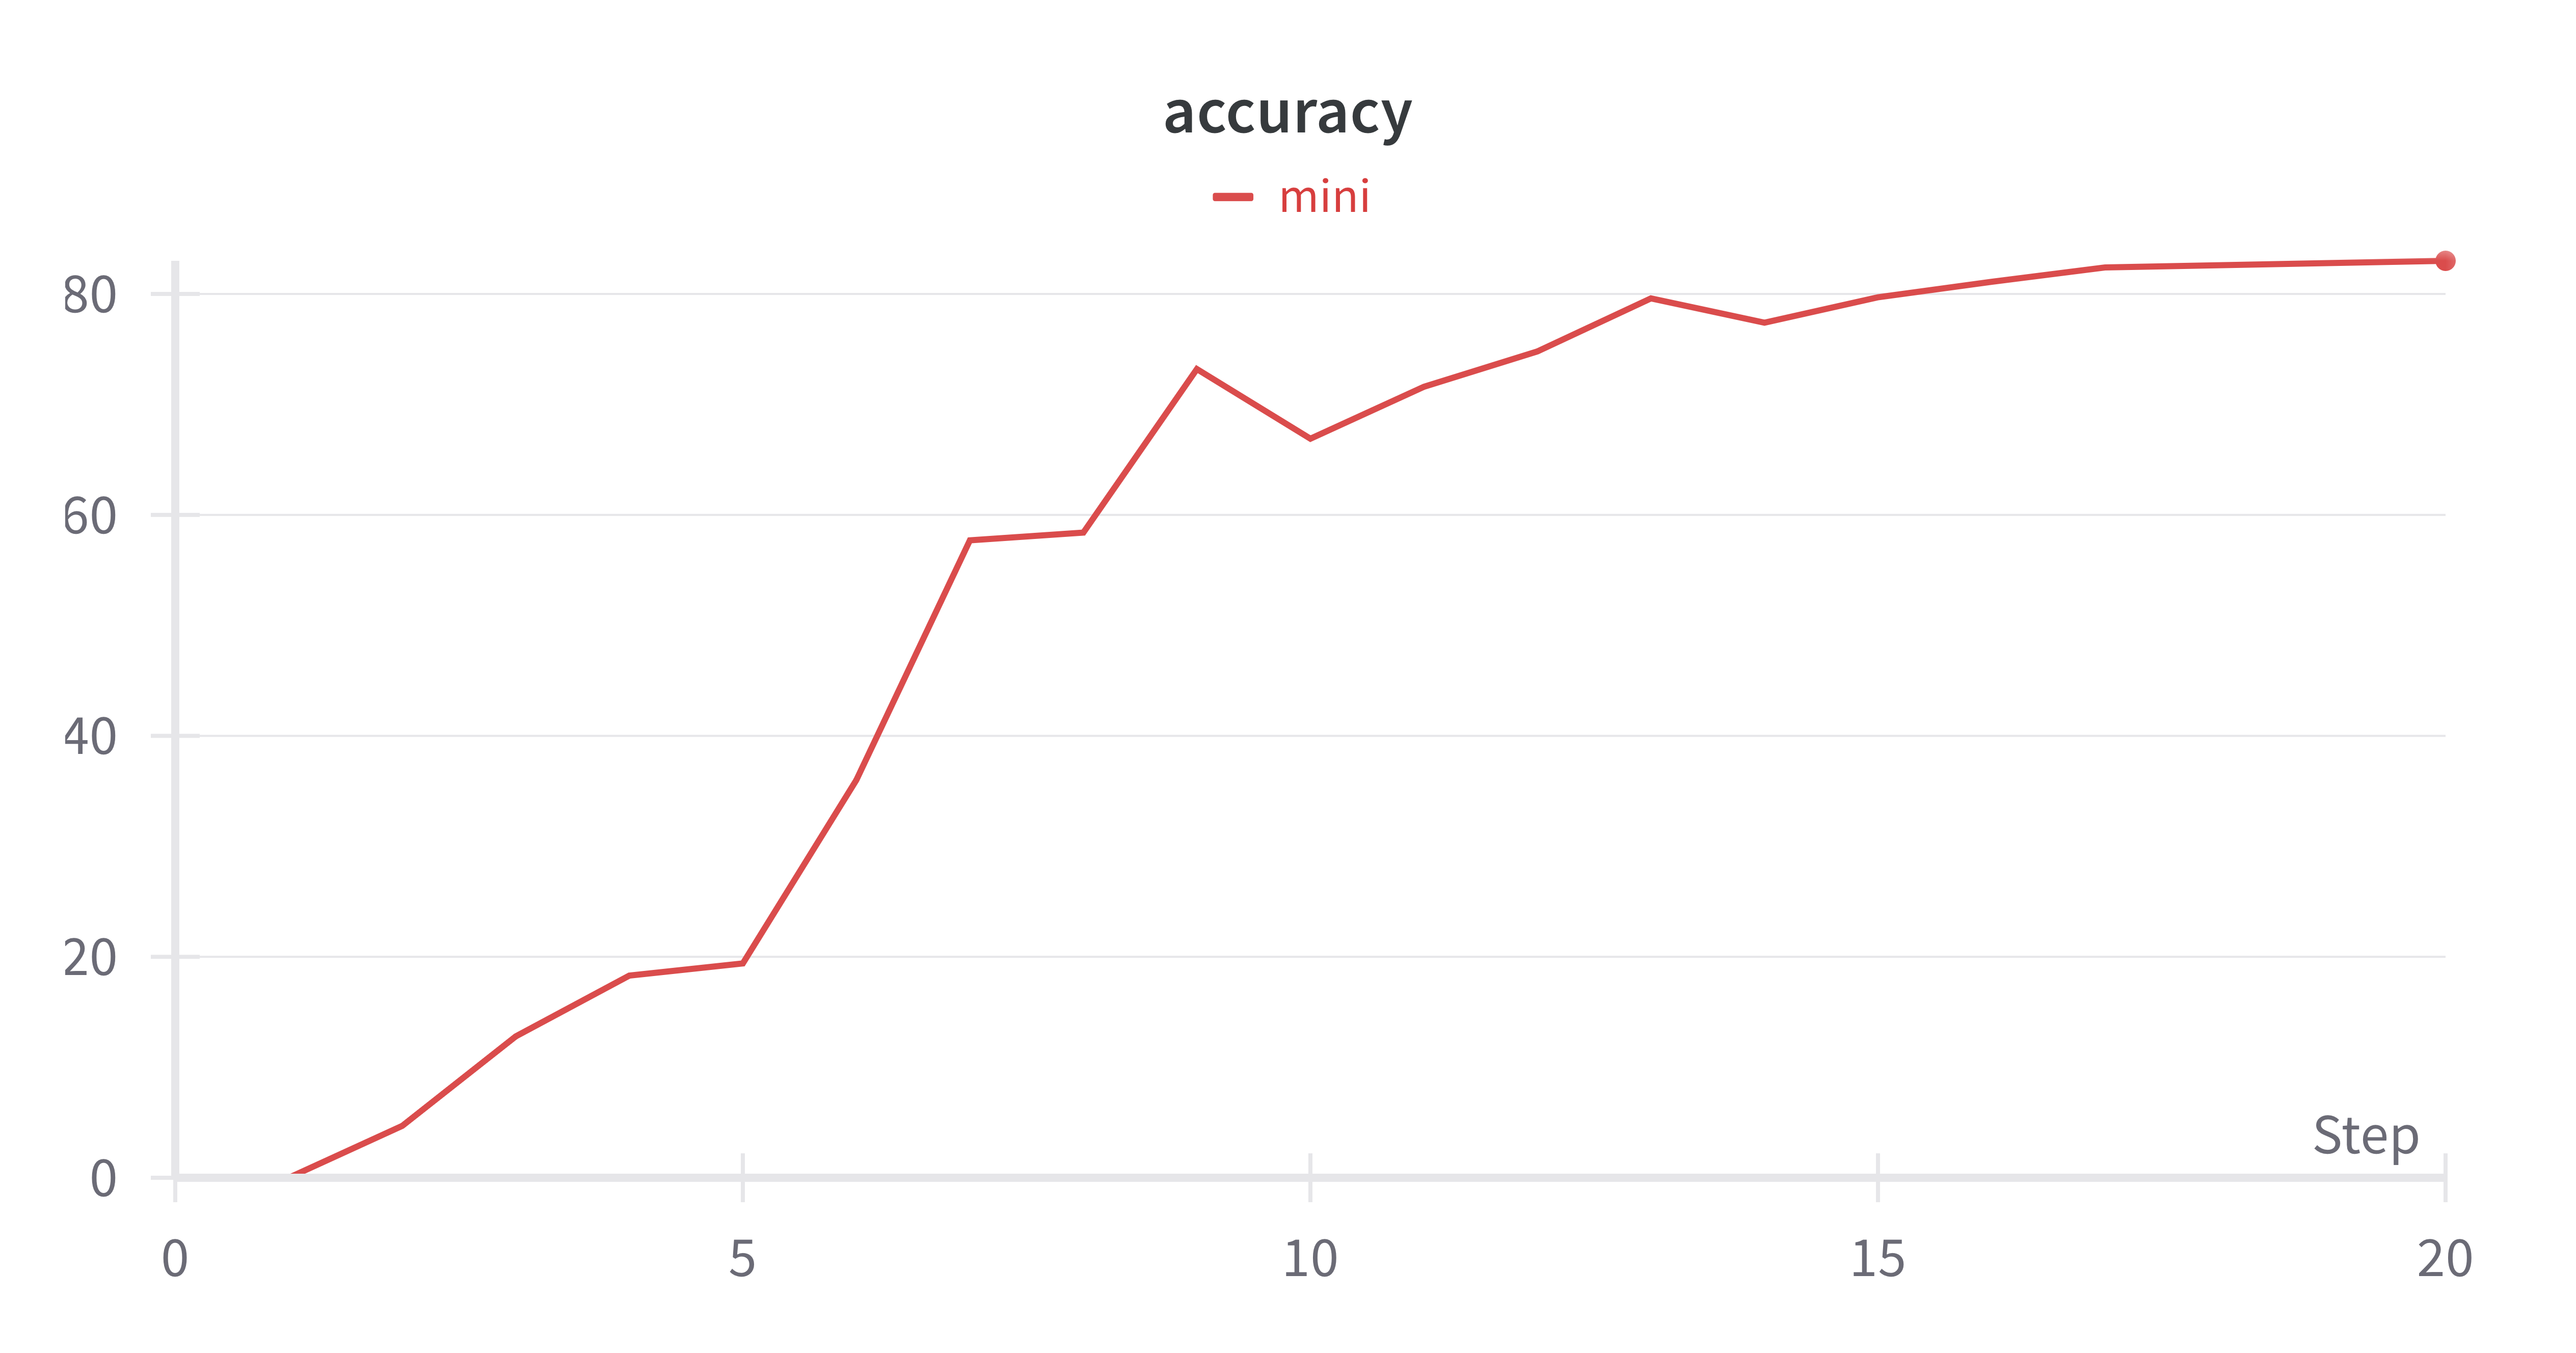
\includegraphics[width=0.5\textwidth]{figures/three-digit/three-digit-add-accuracy.png}
    \caption{Accuracy.}
    \label{fig:three_digit_addition_accuracy}
\end{figure}
\begin{figure}[h]
    \centering
    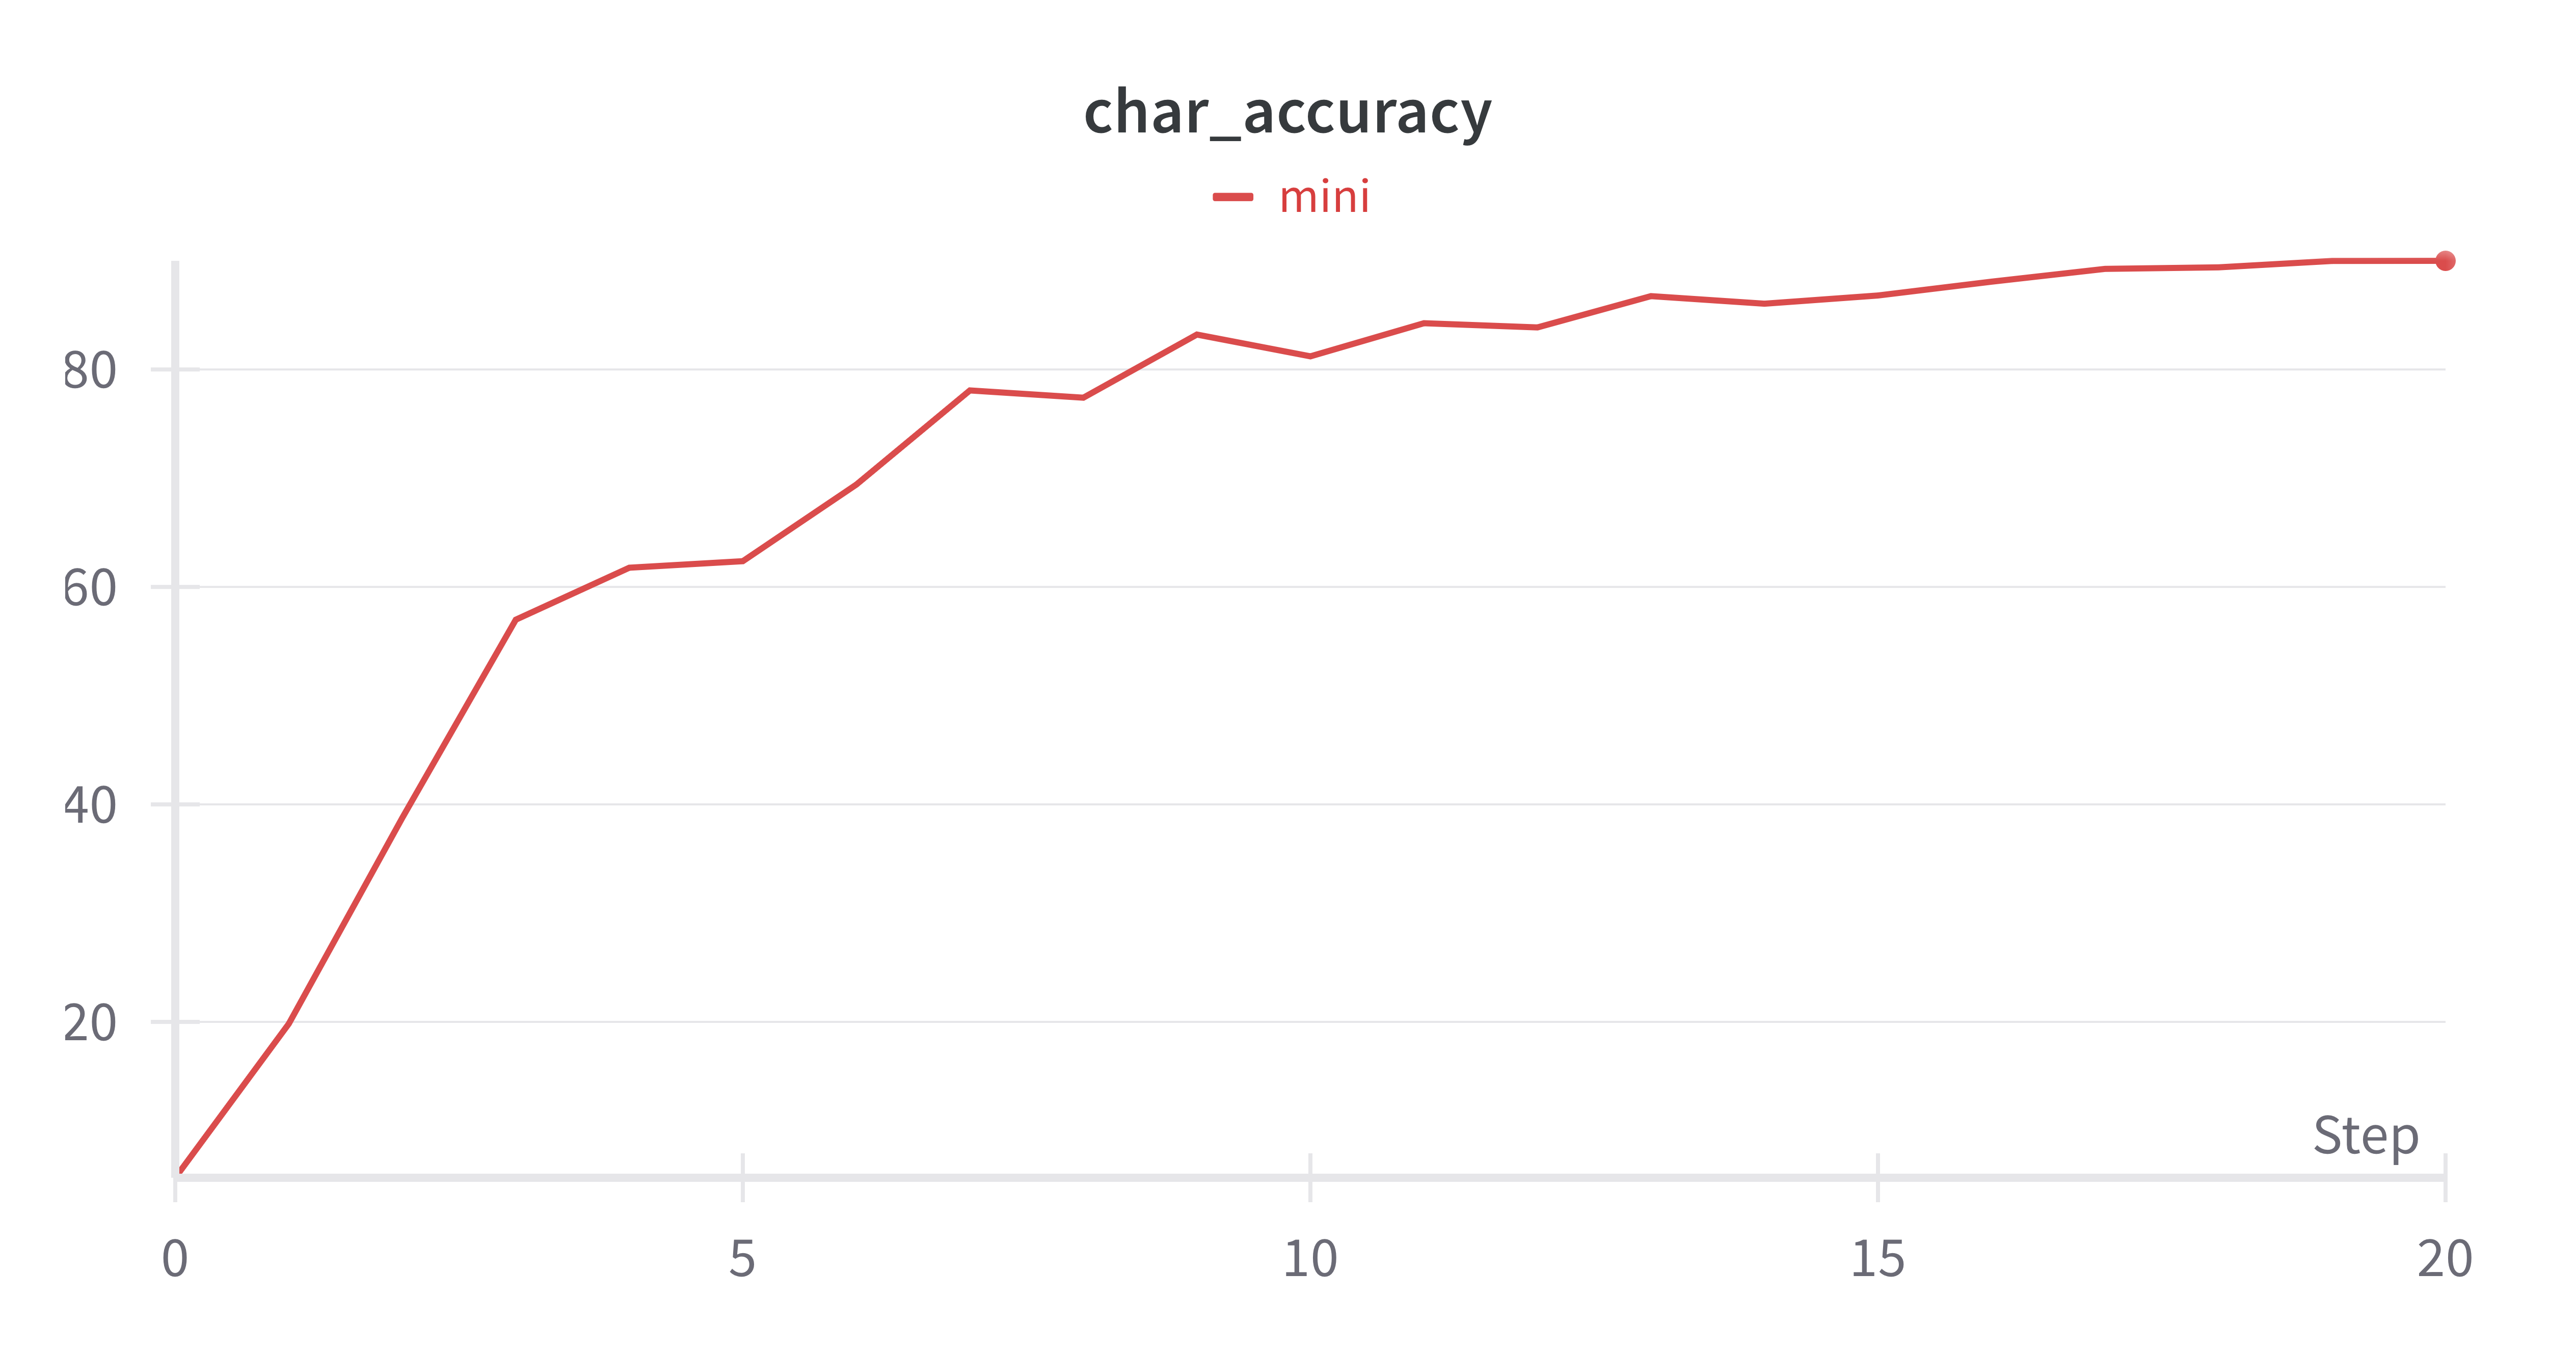
\includegraphics[width=0.5\textwidth]{figures/three-digit/three-digit-add-char-accuracy.png}
    \caption{Character accuracy.}
    \label{fig:three_digit_addition_char_accuracy}
\end{figure}
Figures for training loss, accuracy, and character accuracy are shown in Figures \ref{fig:three_digit_addition}, \ref{fig:three_digit_addition_accuracy}, and \ref{fig:three_digit_addition_char_accuracy} respectively.
Each step is 250 iterations.
We see the same exponential growth in accuracy, before a plateau around 80\%, in line with the results of \cite{lee2023teaching}.
The character accuracy now significantly leads the accuracy, and plateaus around 90\%.
Notably, it has the opposite concavity.
We suspect that if we evaluated the model more frequently near the beginning of training, we would see a similar exponential growth in character accuracy.
\subsection{Reversed Three Digit Addition}
\subsubsection{Random Block Sampling}
Contrary to the results of \cite{lee2023teaching}, we find that the model fails to learn the reversed three digit addition task using random block sampling.
As shown in the figures, the training loss plateaus after a short while, along with the character accuracy.
The accuracy stays extremely low at around 0.1\%.
We are not sure why this is the case, but suspect a data processing issue.
\begin{figure}[h]
    \centering
    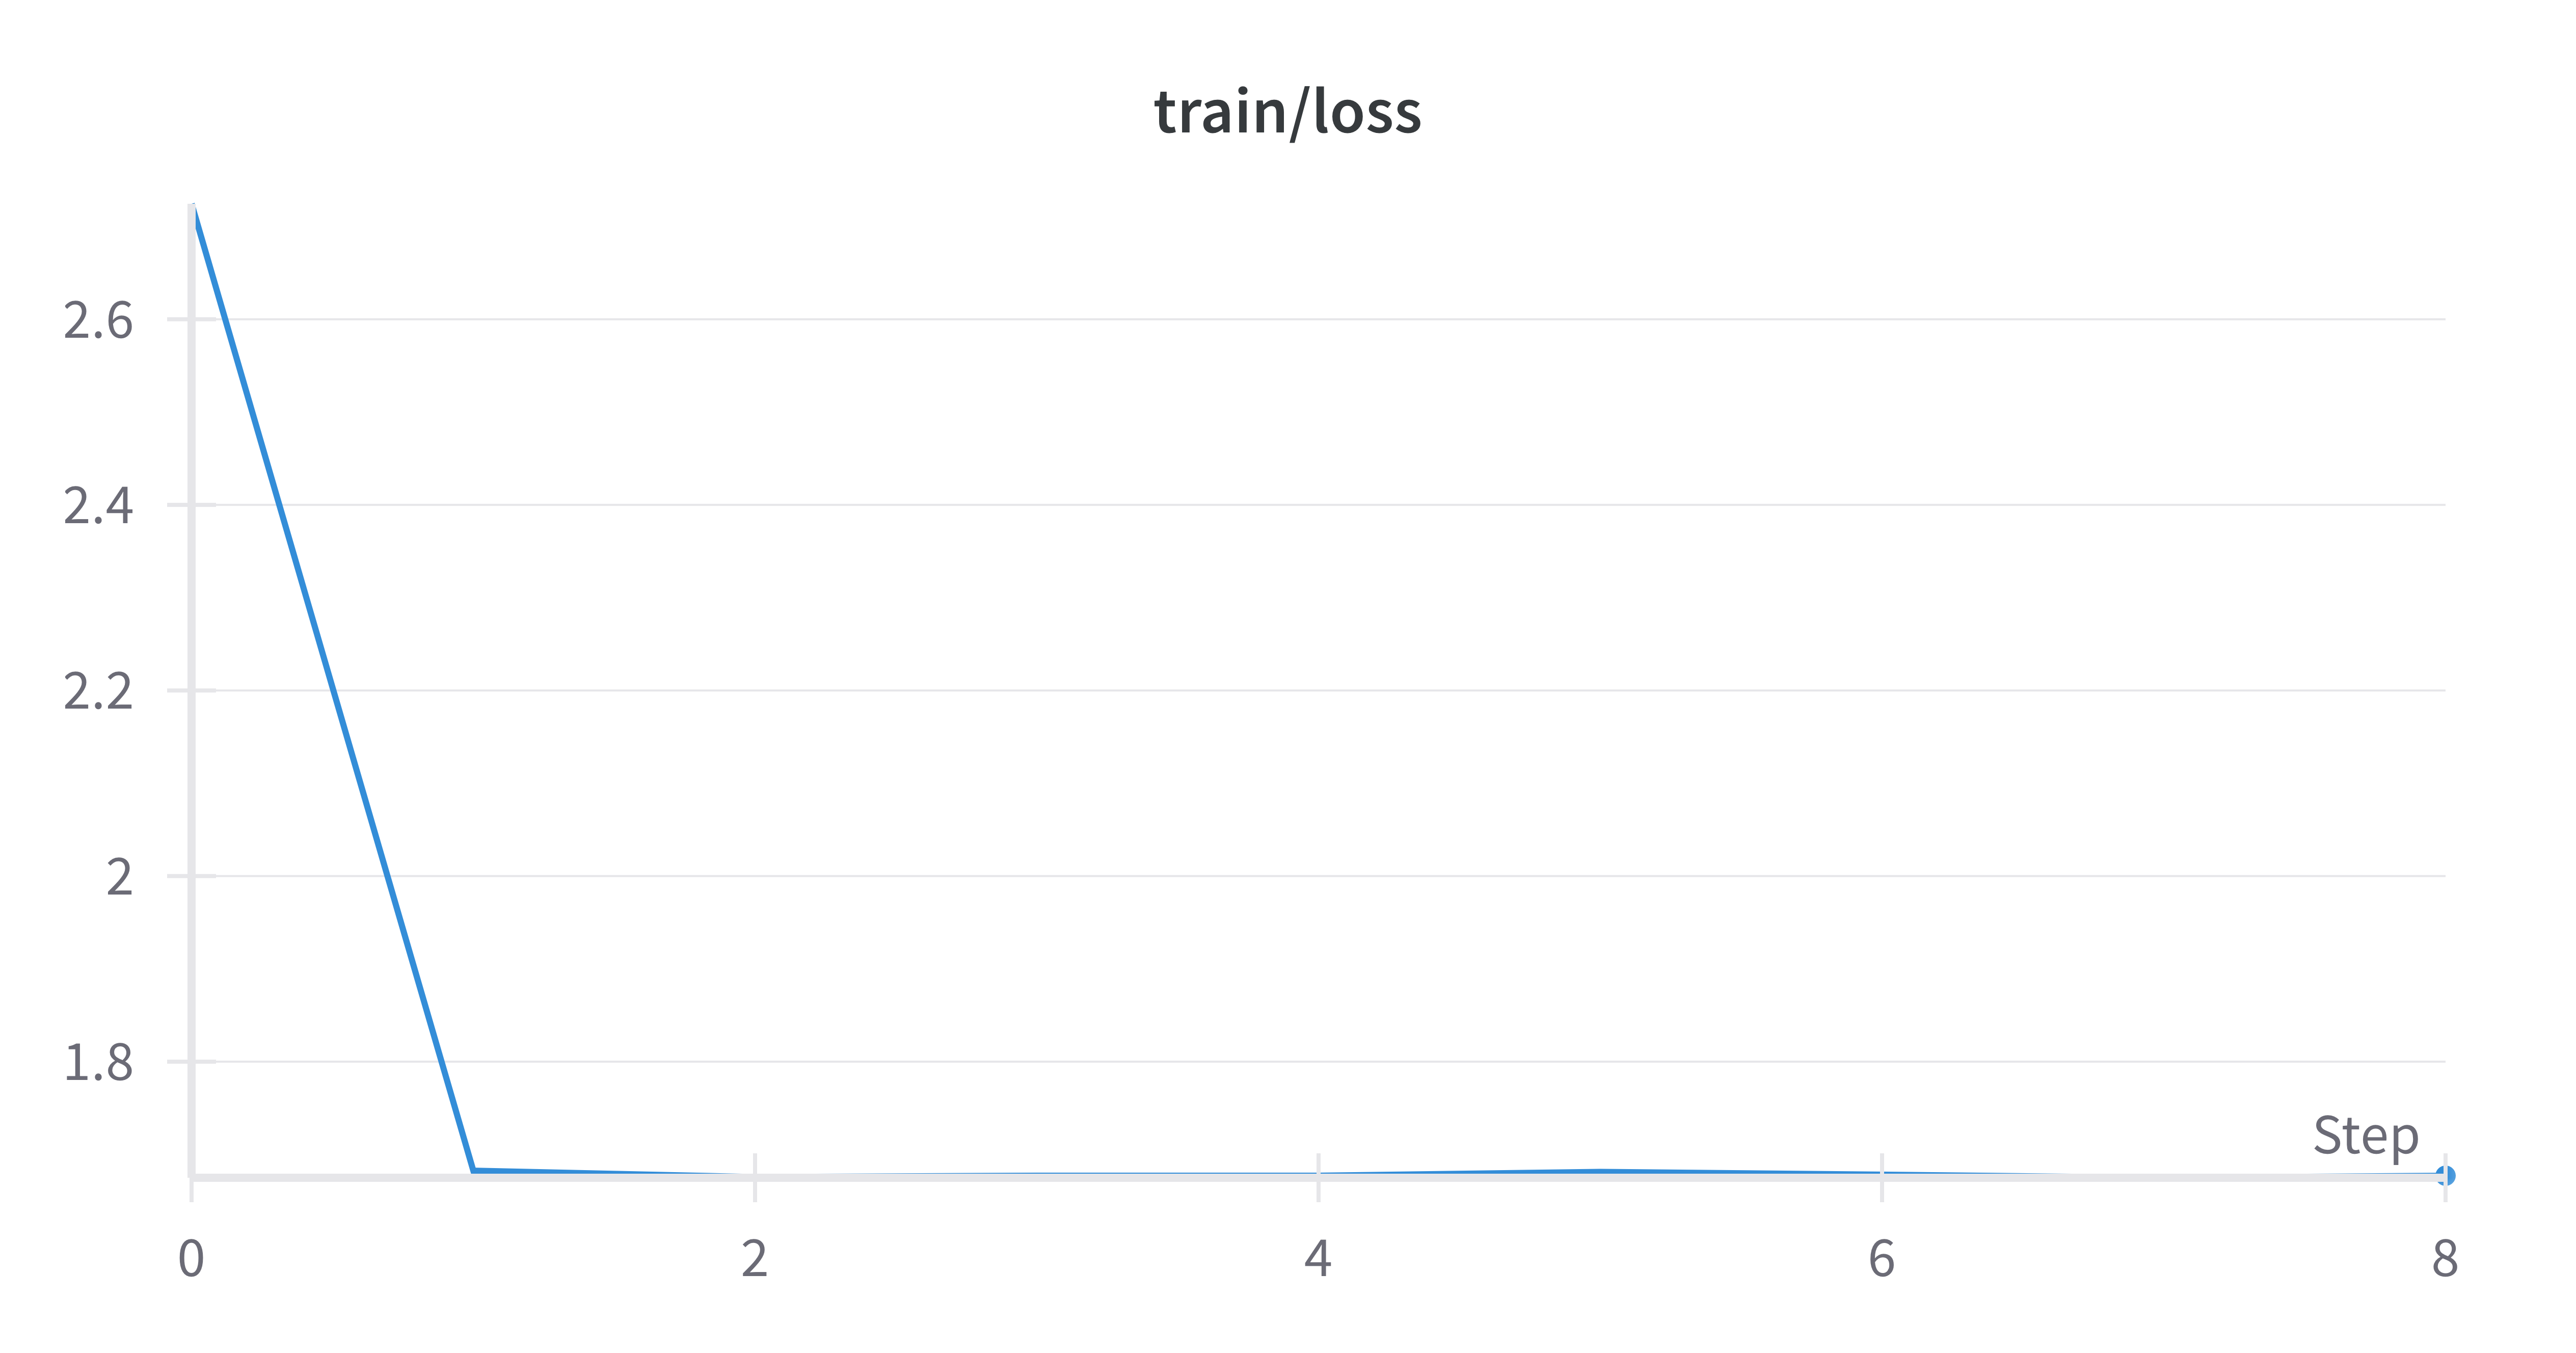
\includegraphics[width=0.5\textwidth]{figures/three-digit-reverse/three-digit-reverse-loss.png}
    \caption{Training loss.}
    \label{fig:reversed_three_digit_addition}
\end{figure}
\begin{figure}[h]
    \centering
    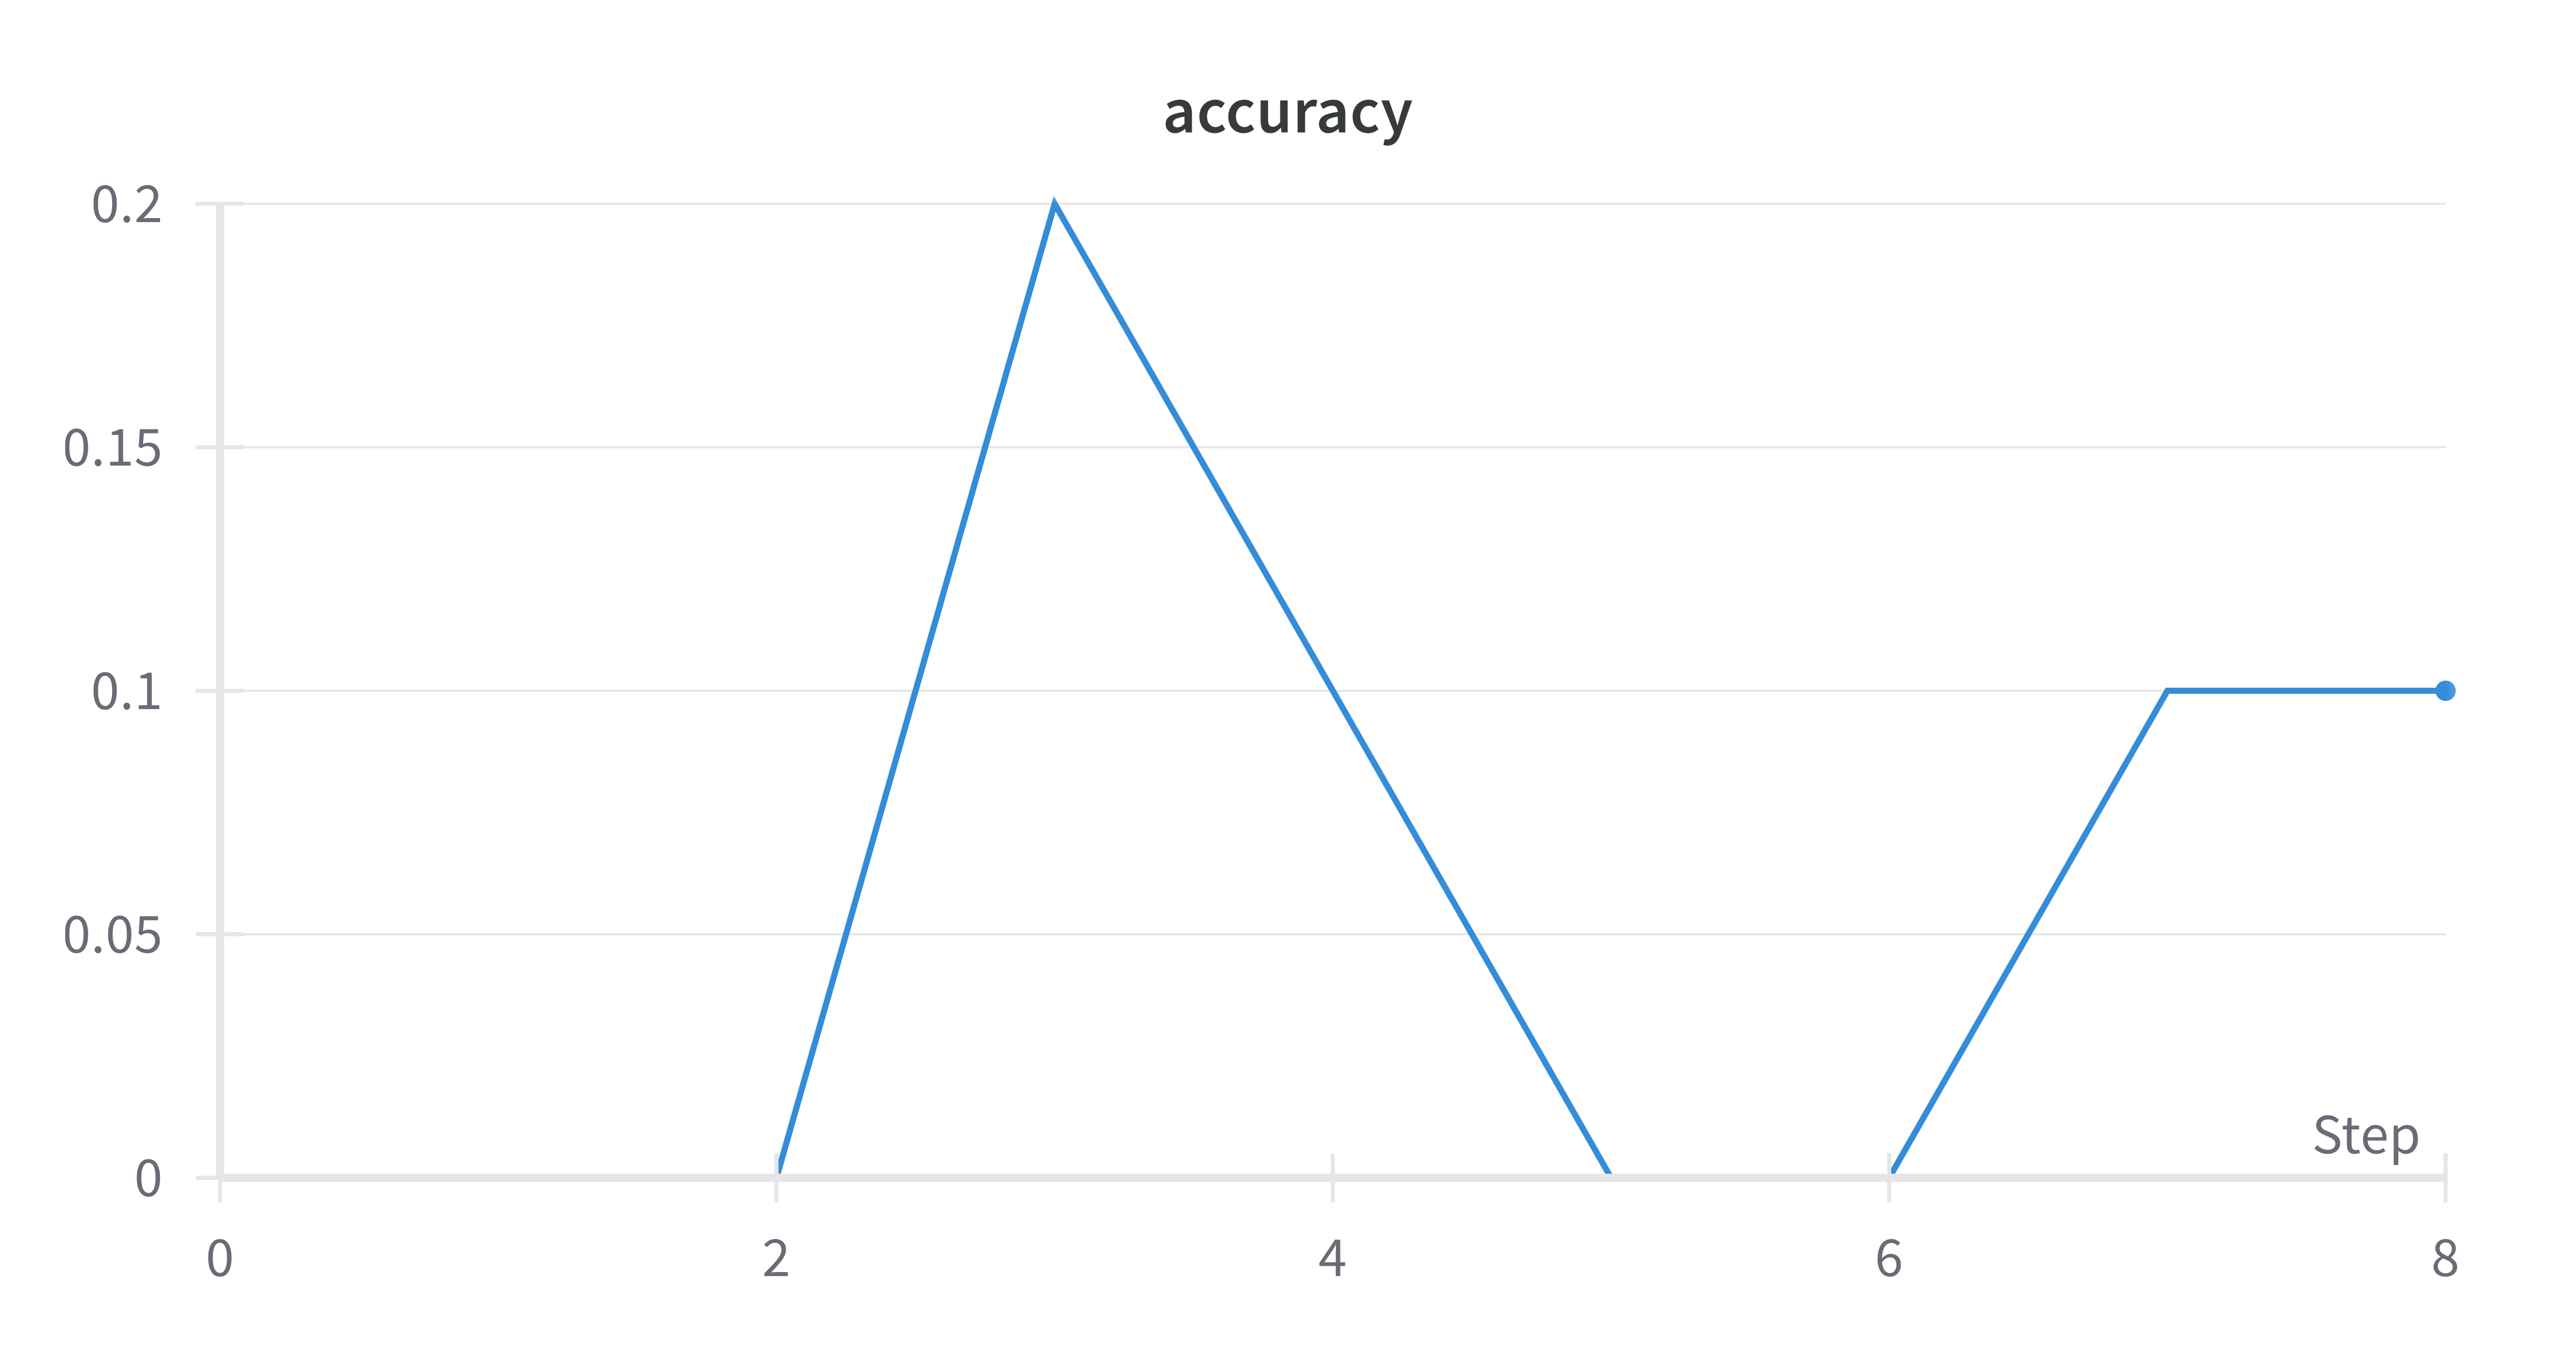
\includegraphics[width=0.5\textwidth]{figures/three-digit-reverse/three-digit-reverse-accuracy.png}
    \caption{Accuracy.}
    \label{fig:reversed_three_digit_addition_accuracy}
\end{figure}
\begin{figure}[h]
    \centering
    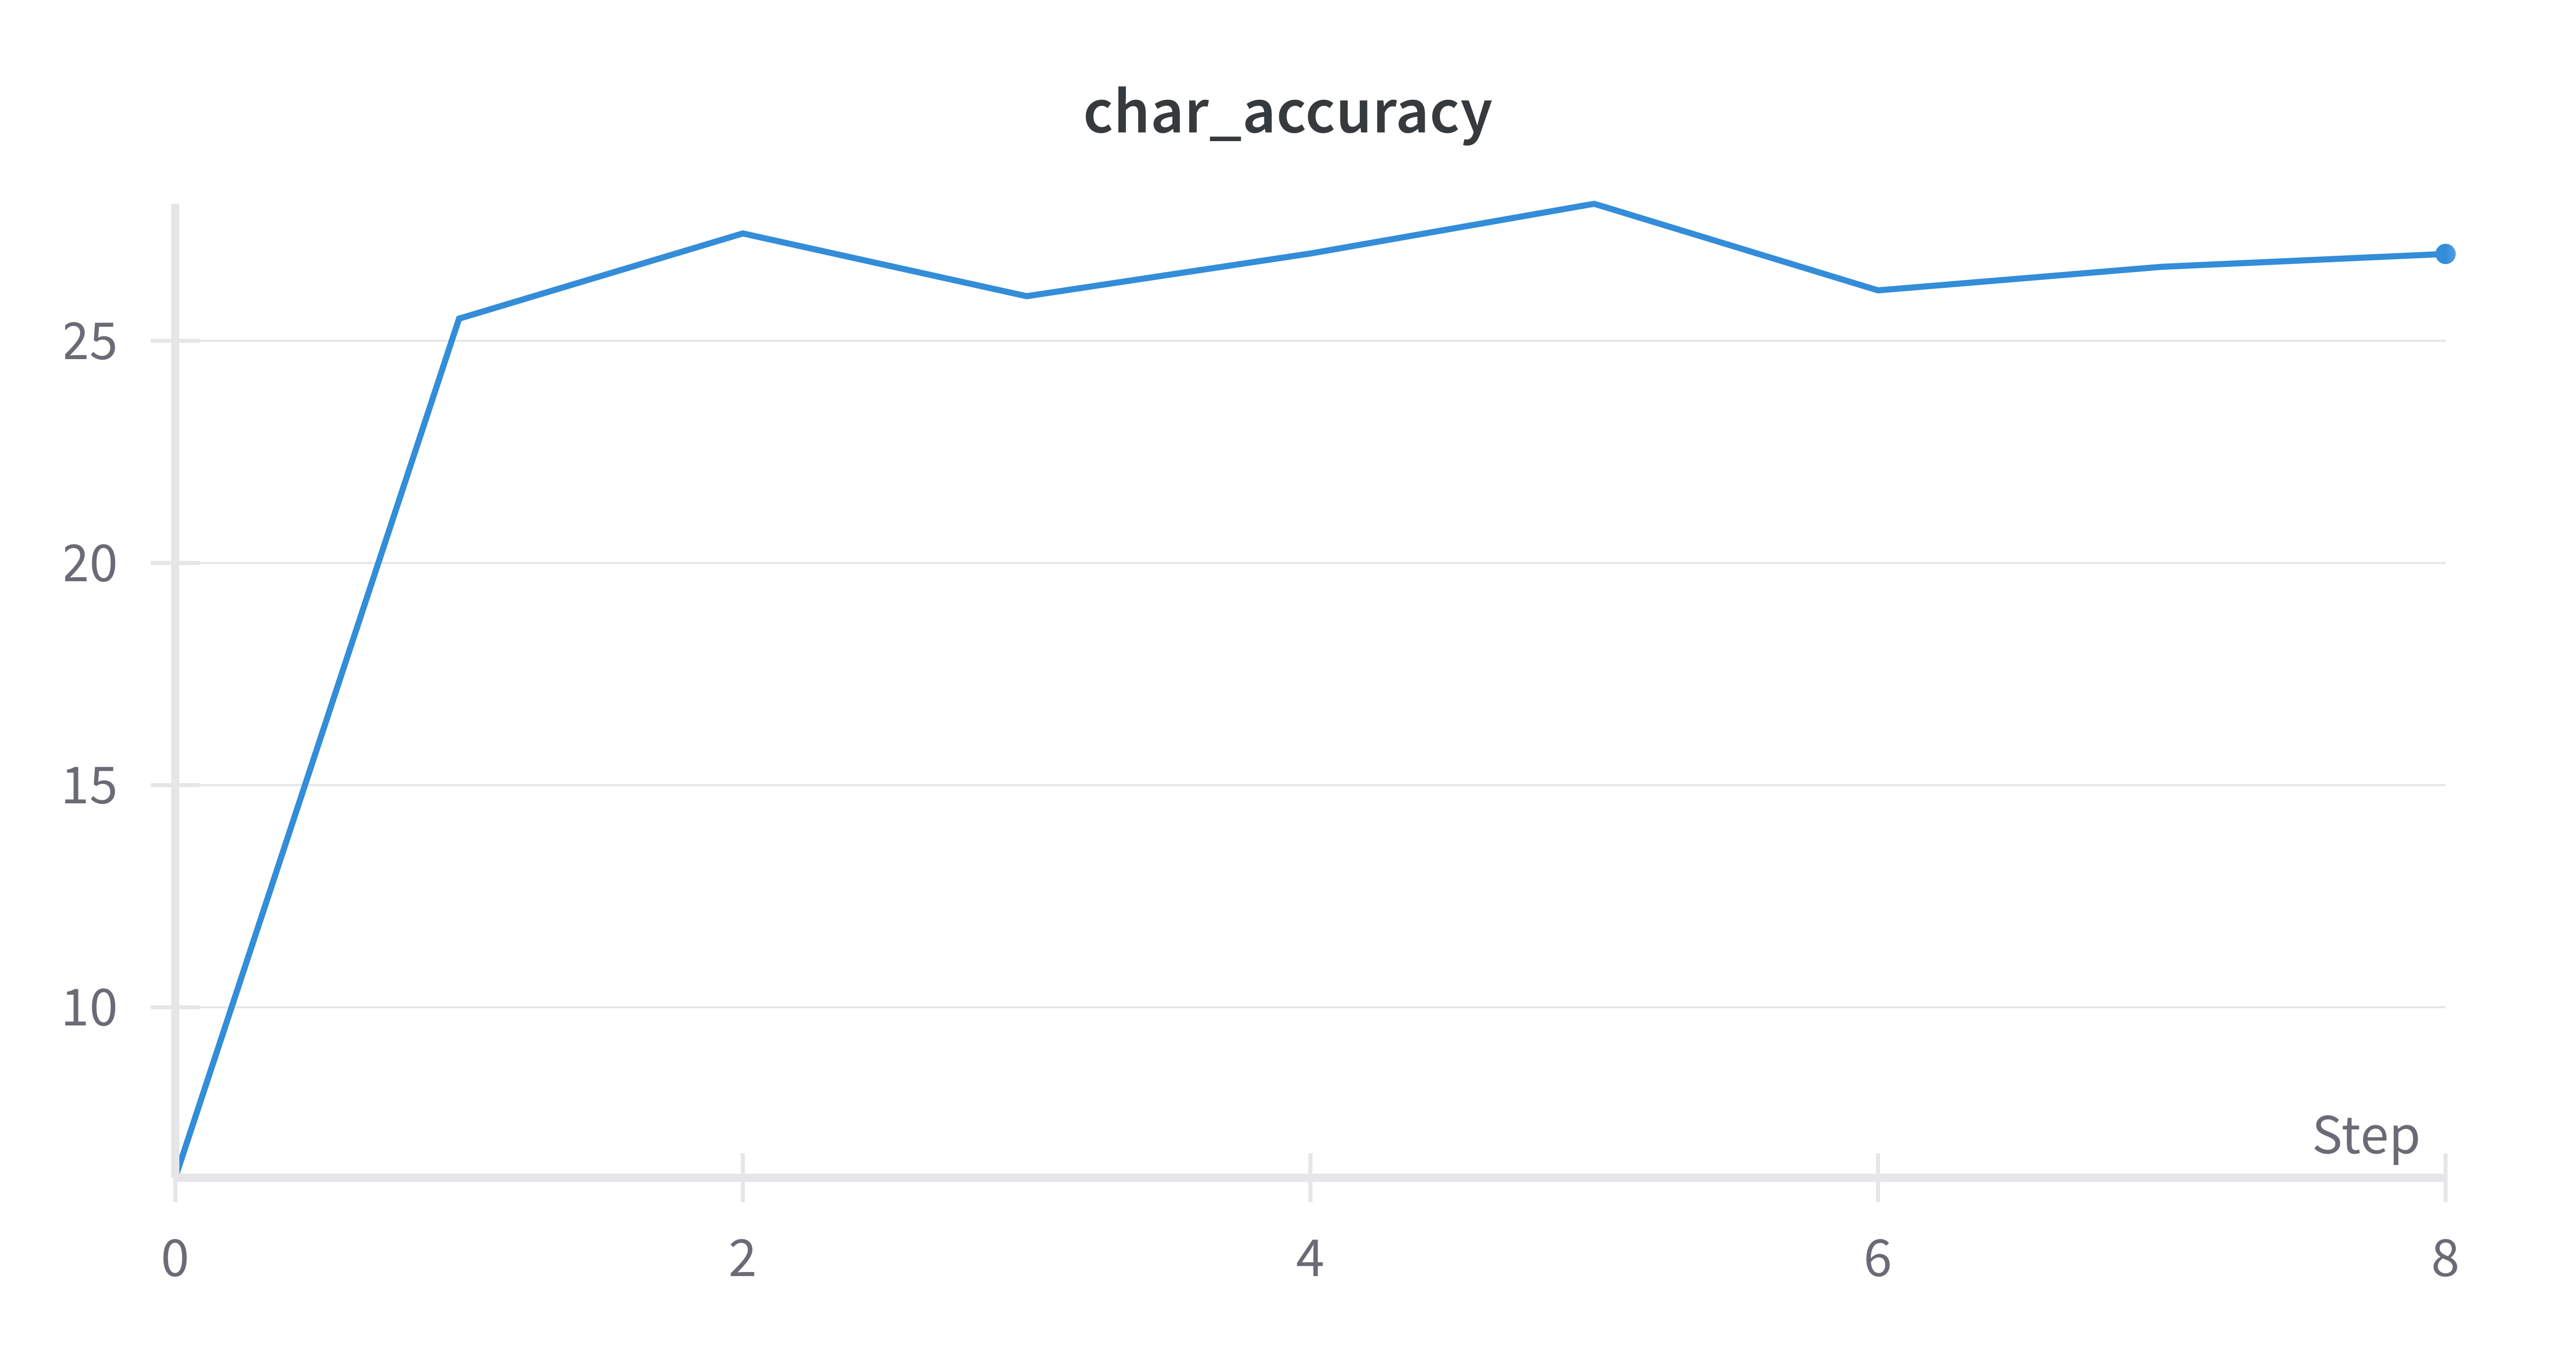
\includegraphics[width=0.5\textwidth]{figures/three-digit-reverse/three-digit-reverse-char-accuracy.png}
    \caption{Character accuracy.}
    \label{fig:reversed_three_digit_addition_char_accuracy}
\end{figure}
Each step is 250 iterations.
\subsubsection{Random Line Sampling}
However, using random line sampling, we find that the model is able to learn the reversed three digit addition task.
In line with the results of \cite{lee2023teaching}, we find that the model is able to learn the task, and achieves a character accuracy of around 90\%.
The accuracy increases significantly faster than plain three digit addition, and plateaus around 80\%.
We are unsure how much of this effect is due to the data loading method, and how much is due to the reasons outlined in \cite{lee2023teaching}.
\begin{figure}[h]
    \centering
    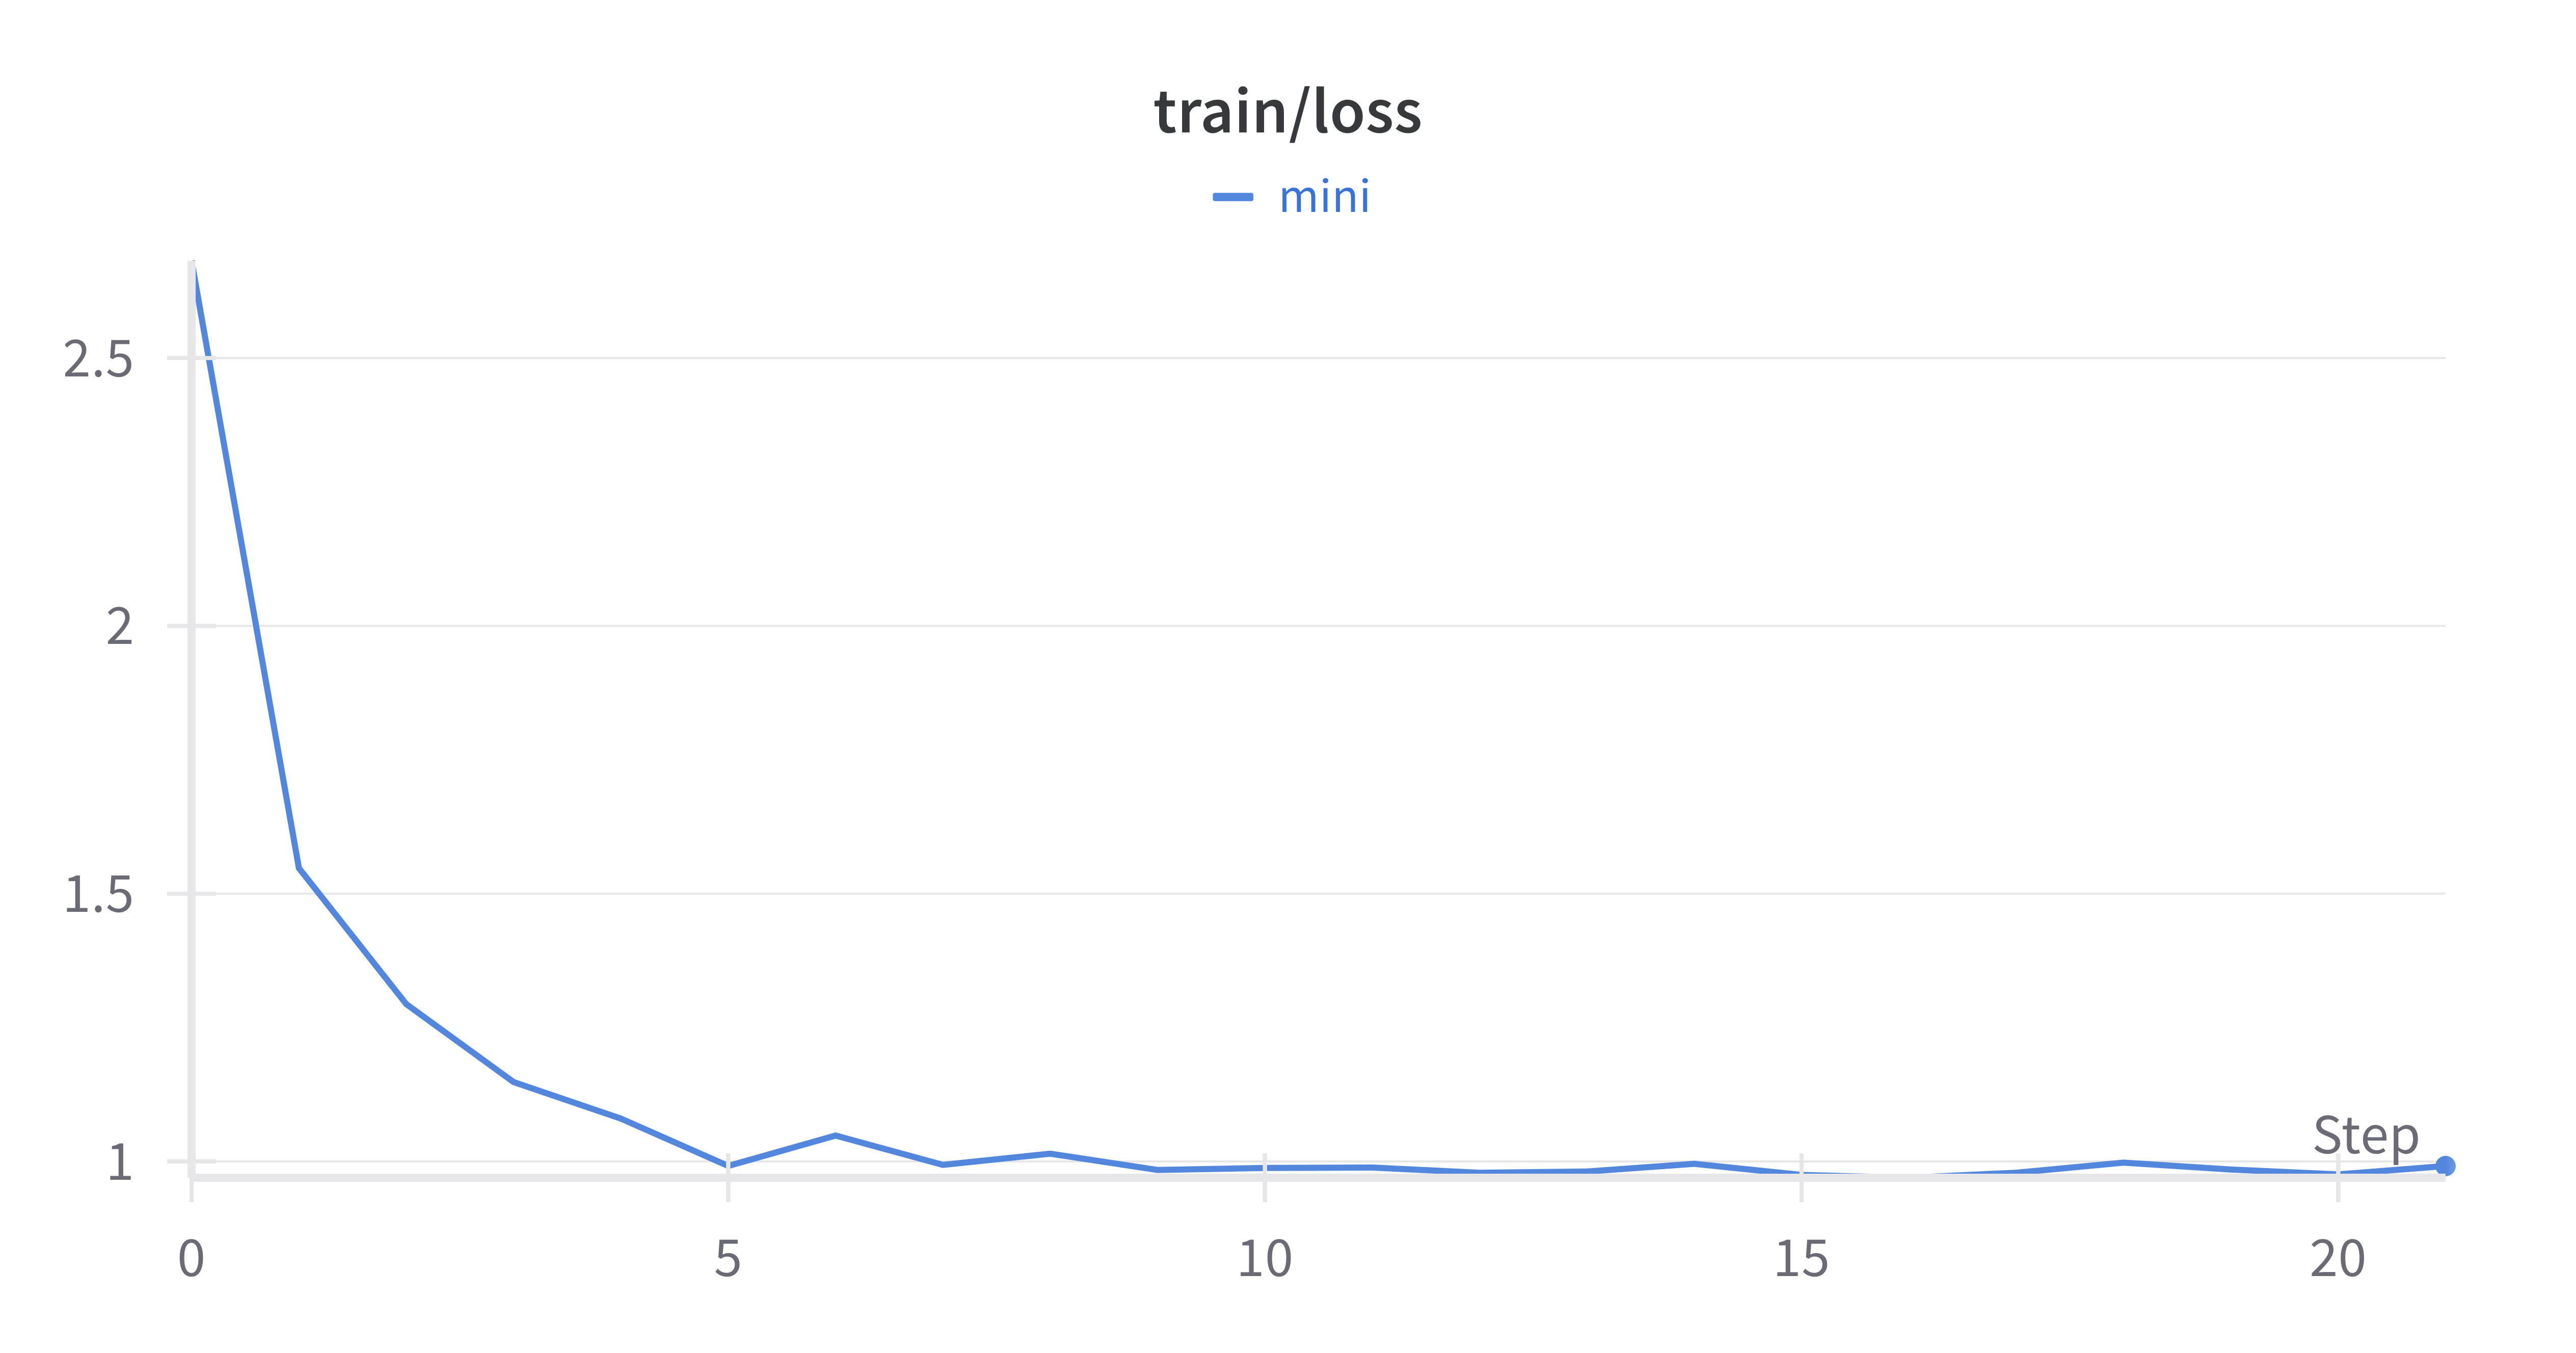
\includegraphics[width=0.5\textwidth]{figures/three-digit-reverse-line/three-digit-add-reverse-line-loss.png}
    \caption{Training loss.}
    \label{fig:reversed_three_digit_addition_line}
\end{figure}
\begin{figure}[h]
    \centering
    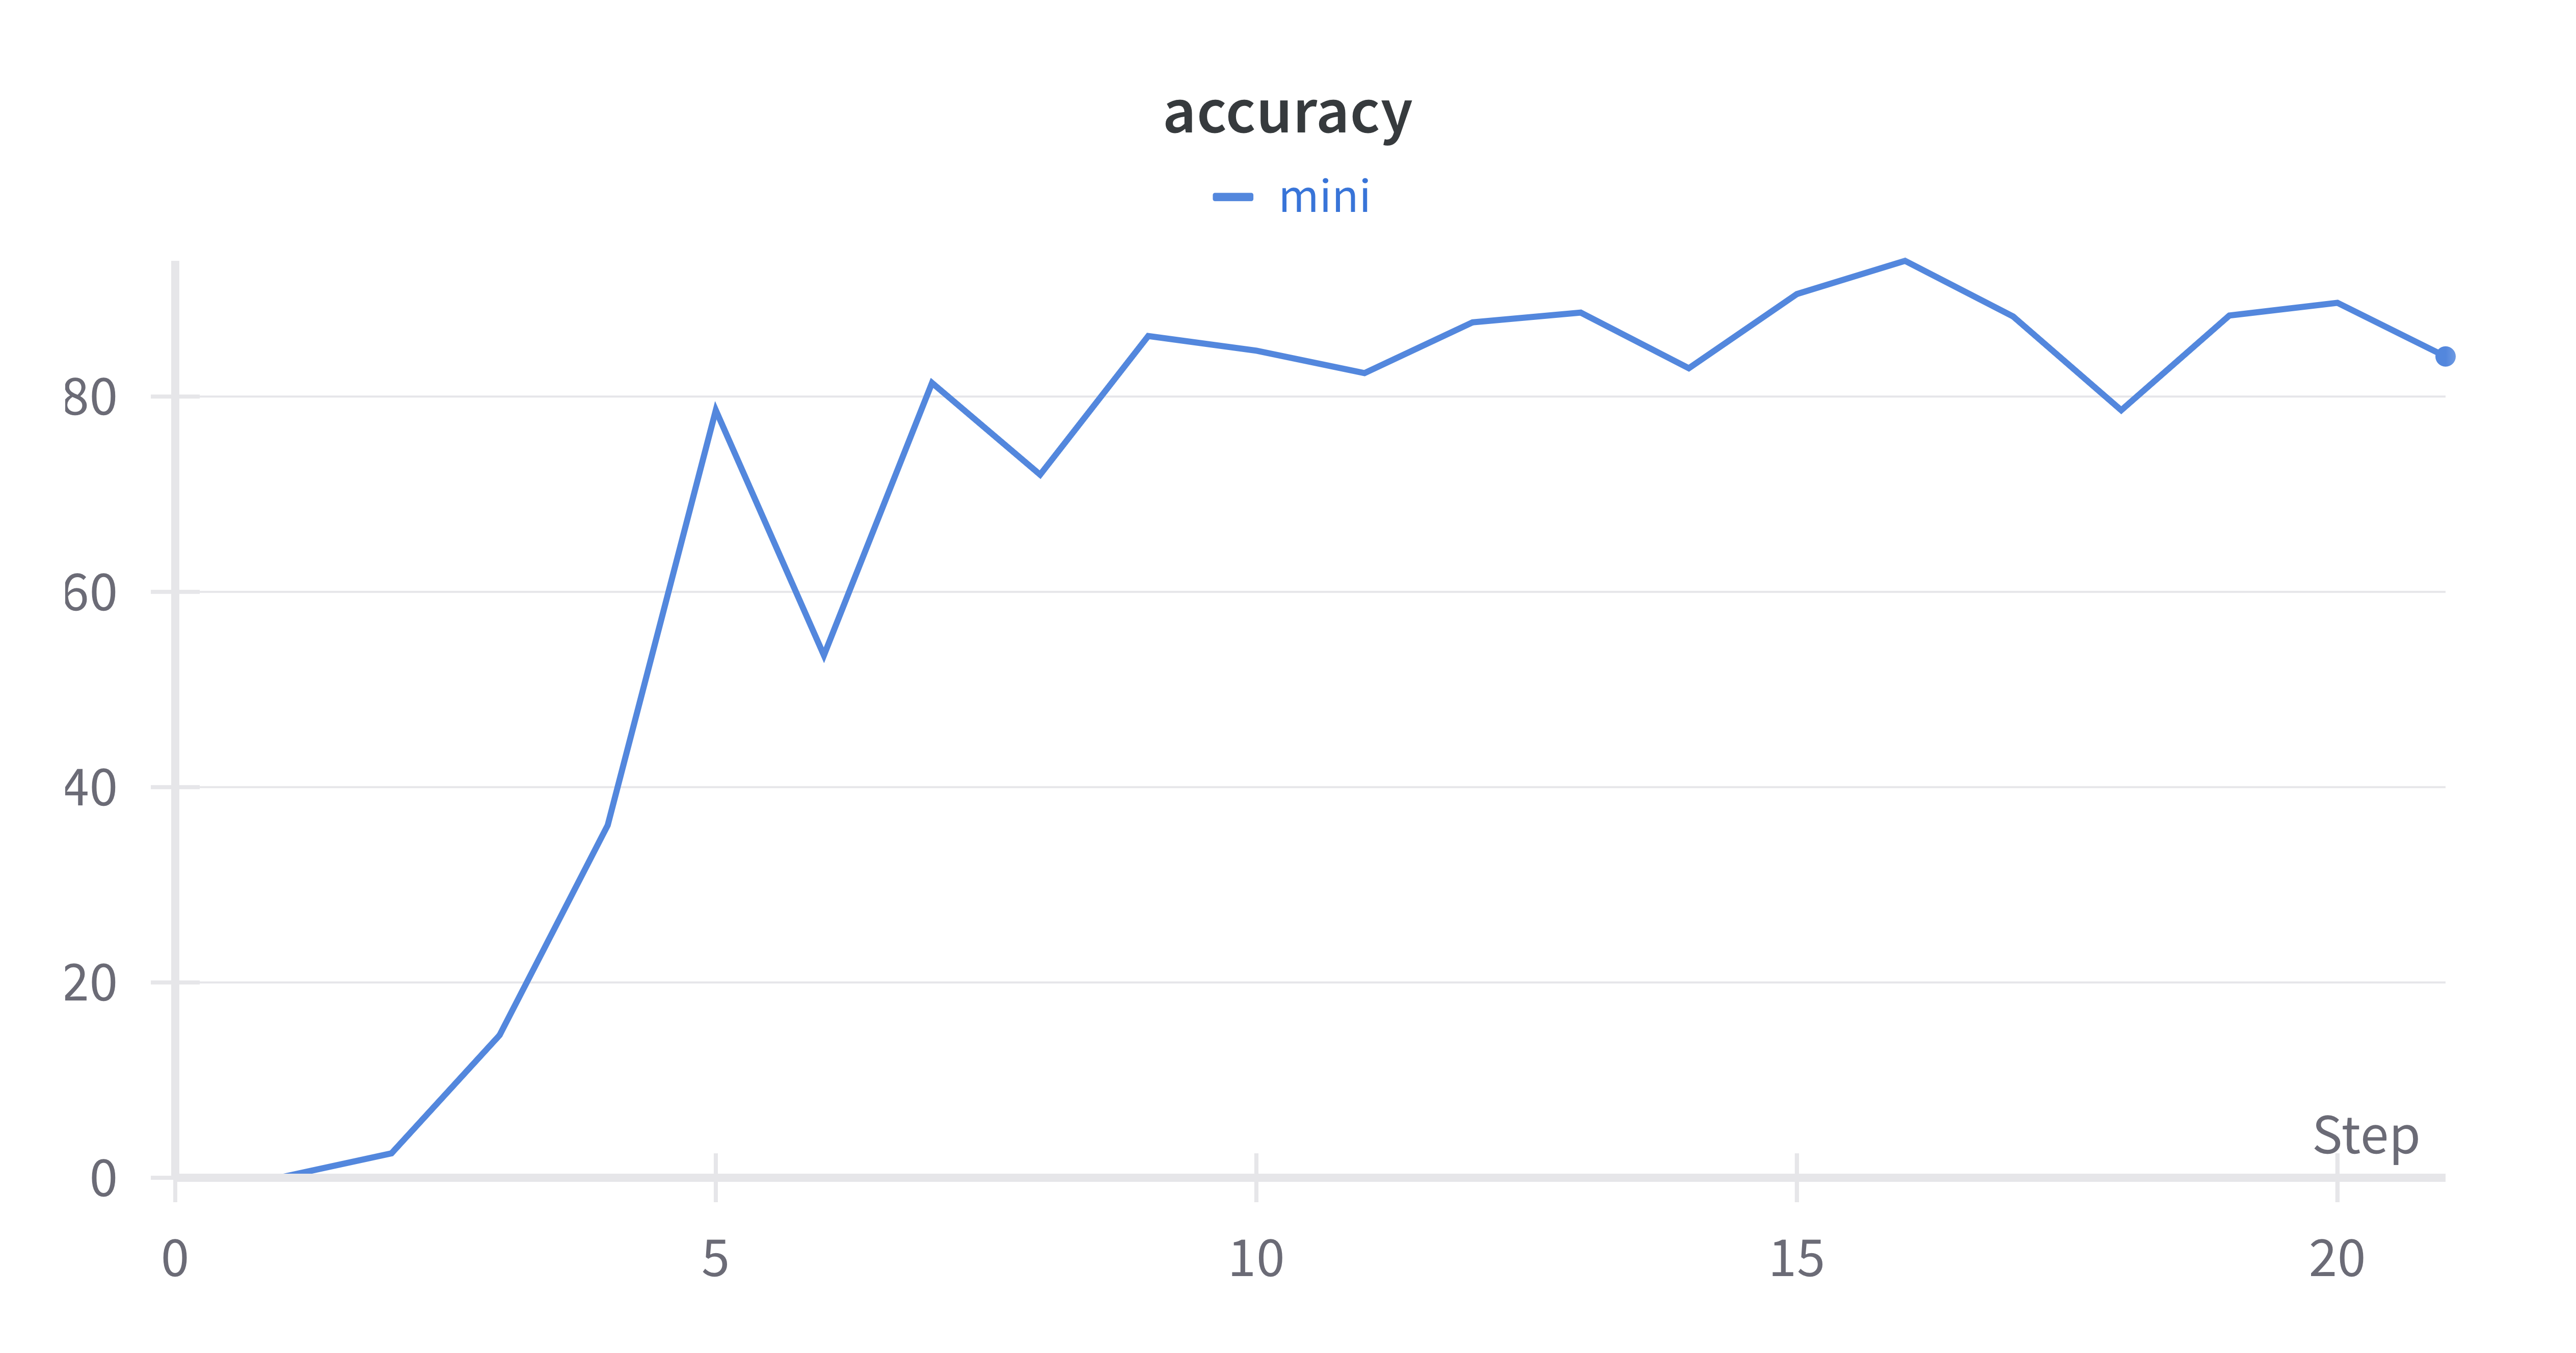
\includegraphics[width=0.5\textwidth]{figures/three-digit-reverse-line/three-digit-add-reverse-line-accuracy.png}
    \caption{Accuracy.}
    \label{fig:reversed_three_digit_addition_accuracy_line}
\end{figure}
\begin{figure}[h]
    \centering
    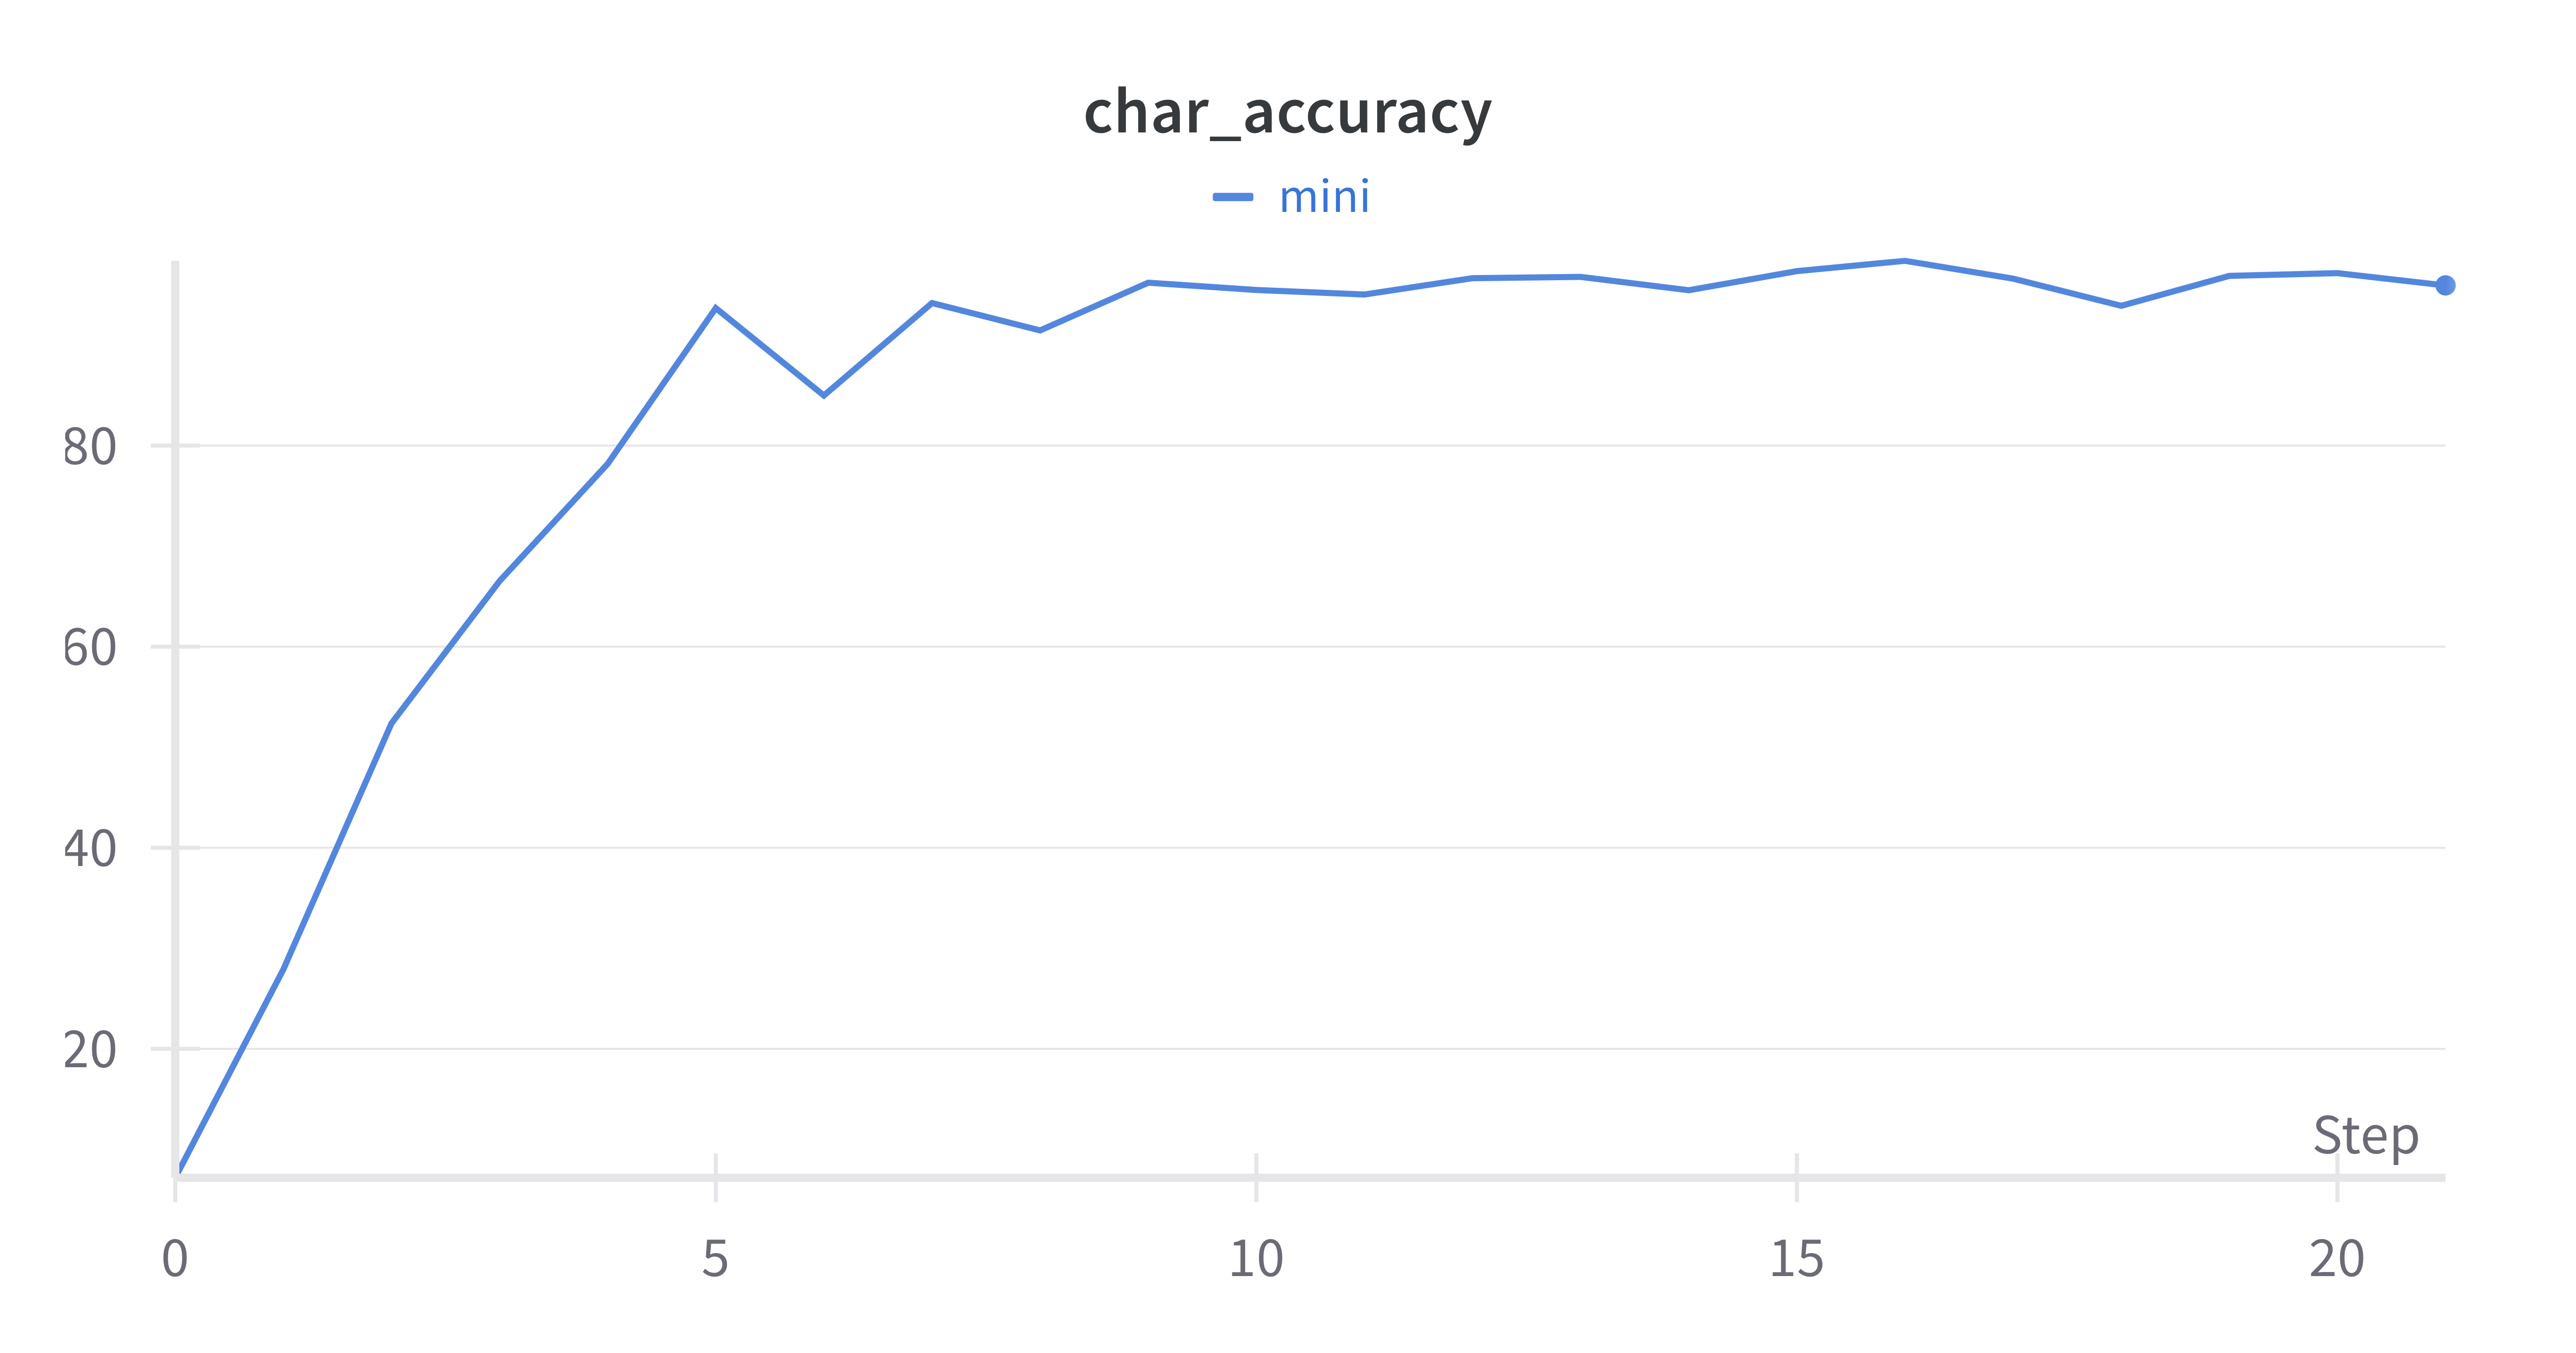
\includegraphics[width=0.5\textwidth]{figures/three-digit-reverse-line/three-digit-add-reverse-line-char-accuracy.png}
    \caption{Character accuracy.}
    \label{fig:reversed_three_digit_addition_char_accuracy_line}
\end{figure}
Each step is 250 iterations.
\section{Conclusion}
In this report, we have managed to mostly replicate the results of \cite{lee2023teaching}.
Possible future work includes:
\begin{itemize}
    \item Investigating the model's performance on other arithmetic tasks, such as multiplication and division.
    \item Using random line sampling for the three digit addition dataset.
    \item Investigating the types of errors the model makes, such as whether they tend to mispredict digits by one.
\end{itemize}

\bibliographystyle{plainurl}
\bibliography{references}

\end{document}